\documentclass[11pt]{article}
\usepackage[margin=0.82in]{geometry}
\usepackage[T1]{fontenc}
\usepackage[utf8]{inputenc}
\usepackage{lmodern}
\usepackage{amsmath,amssymb}
\usepackage{graphicx}
\usepackage{booktabs}
\usepackage{tabularx}
\usepackage{array}
\usepackage{pdflscape}
\usepackage{float}
\IfFileExists{algpseudocode.sty}{\usepackage{algorithm}\usepackage[noend]{algpseudocode}}{% Minimal algorithm layout, using only the standard list and float packages.
\floatstyle{ruled}
\newfloat{algorithm}{htbp}{loa}
\floatname{algorithm}{Algorithm}
\newcounter{algline}
\newcounter{algdepth}
\newcommand{\algorithmicrequire}{\textbf{Input:}}
\newcommand{\algorithmicensure}{\textbf{Output:}}
\let\algrenewcommand\renewcommand
\newenvironment{algorithmic}[1][]{%
\setcounter{algline}{0}\setcounter{algdepth}{0}%
\begin{list}{}{\setlength{\leftmargin}{2.1em}\setlength{\labelwidth}{1.6em}\setlength{\labelsep}{.5em}\setlength{\itemsep}{.12em}\setlength{\parsep}{0pt}\setlength{\topsep}{.4em}}%
}{\end{list}}
\newcommand{\State}{\stepcounter{algline}\item[\scriptsize\arabic{algline}:]\hspace*{\value{algdepth}em}}
\newcommand{\Require}{\item[]\algorithmicrequire\ }
\newcommand{\Ensure}{\item[]\algorithmicensure\ }
\newcommand{\ForAll}[1]{\State\textbf{for all} #1 \textbf{do}\stepcounter{algdepth}}
\newcommand{\For}[1]{\State\textbf{for} #1 \textbf{do}\stepcounter{algdepth}}
\newcommand{\If}[1]{\State\textbf{if} #1 \textbf{then}\stepcounter{algdepth}}
\newcommand{\Else}{\addtocounter{algdepth}{-1}\State\textbf{else}\stepcounter{algdepth}}
\newcommand{\EndFor}{\addtocounter{algdepth}{-1}}
\newcommand{\EndIf}{\addtocounter{algdepth}{-1}}
}
\usepackage{xcolor}
\usepackage{microtype}
\usepackage{hyperref}
\hypersetup{colorlinks=true,linkcolor=blue!55!black,urlcolor=blue!55!black,citecolor=blue!55!black}
\setlength{\parindent}{0pt}
\setlength{\parskip}{0.55em}
\algrenewcommand\algorithmicrequire{\textbf{Input:}}
\algrenewcommand\algorithmicensure{\textbf{Output:}}

\title{Computational Supplement:\\Correlation Emergence and the Epps Effect}
\author{Chris Angstmann \and Tim Gebbie}
\date{v2.2.0 --- Numerical resolution update\\12 September 2026}

\begin{document}
\maketitle

\begin{abstract}
This supplement records the analytical and simulation companion to ``Correlation emergence and the Epps effect in two coupled limit order books'' (arXiv:2606.14182). It evaluates the paper's ordinary and fractional correlation build-up factors, reports their sensitivities and identifiability limits, diagnoses finite-grid boundary representation, and verifies a uniform-operational simulation followed by explicit book-specific previous-refresh subordination. The numerical evidence includes clock-only and translation-mode coupling comparisons, a combined fixed-parameter comparison, single-trade and meta-order impact, mid-price-increment and trade-sign autocorrelations, fixed-time order-book shock recovery, and stylised-facts diagnostics. The observation-clock comparison separates exogenous long-memory order flow from Poisson, Mittag--Leffler and exponentially tempered observation clocks, then measures paired single-trade and meta-order impact in each domain. This numerical resolution update increases independent simulation depth, refines the impact grid, and reports group-aware mean uncertainty. The computations are model-conditional reproducibility evidence, not empirical calibration or mathematical proof.
\end{abstract}

\tableofcontents

\section{Scientific scope}

The frozen source paper remains the mathematical source of truth. The simulation implementation preserves that source snapshot. The ordinary clock, coupling, and combined curves remain illustrations of the paper's renewal-envelope, exponential-response, and leading-order separability assumptions. The fractional curves evaluate the stated Mittag--Leffler replacement on the non-negative real axis. The reaction-boundary implementation uses the decaying Gaussian convention for which the paper gives a finite half-line moment.

Market-data calibration and trading use are outside the scope of these computations. The antecedent implementation of Bauer et al. motivates the source-convention and boundary-representation distinctions below; it is not an executable dependency. Scientific attribution is retained independently of software development history.

Figures 7, 9--11, 13 and 14 use the v2.2.0 ensembles and presentation described here. Figures 1--6, 8 and 12 and the two deterministic benchmark tables retain the published v2.1.0 evidence. Figure 8 therefore retains its independently calibrated covariance normalization; it should not be interpreted as a second rendering of the matched estimator in Figure 7b. No physical parameter was refitted to improve visual agreement.

Both books first evolve on one uniform operational grid. Book-specific calendar clocks act only after the complete operational path exists, by selecting the previous completed state. Calendar waits never enter the density recurrence; no calendar interpolation, extrapolation or nonuniform state update is used.

\section{Theory-to-computation map}

The ordinary build-up kernel is
\begin{equation}
F(x)=1-\frac{1-e^{-x}}{x},\qquad x\geq0,
\label{eq:ordinary}
\end{equation}
with (F(0)=0) defined by continuity. The implementation uses \texttt{expm1} away from the origin and the local series
\begin{equation}
F(x)=\frac{x}{2}-\frac{x^2}{6}+\frac{x^3}{24}-\frac{x^4}{120}+O(x^5)
\end{equation}
near zero. Its derivative and local rate elasticity are
\begin{equation}
F'(x)=\frac{1-(1+x)e^{-x}}{x^2},
\qquad
S_F(x)=\frac{xF'(x)}{F(x)}.
\label{eq:elasticity}
\end{equation}

The normalised ordinary components are
\begin{align}
C_{\mathrm{clock}}(\Delta)&=F(\lambda_{12}\Delta),\\
C_{\mathrm{coupling}}(\Delta)&=F(\kappa\Delta),\\
C_{\mathrm{combined}}(\Delta)&=C_{\mathrm{clock}}(\Delta)C_{\mathrm{coupling}}(\Delta).
\end{align}
The last expression is the paper's leading-order factorisation; the calculation does not promote it to an exact independence result.

For a characteristic time \(\tau\), the fractional component is written
\begin{equation}
F_\alpha(\Delta;\tau)
=1-E_{\alpha,2}\!\left[-(\Delta/\tau)^\alpha\right],
\qquad 0<\alpha\leq1.
\label{eq:fractional}
\end{equation}
The release evaluator uses a deterministic real-axis quadrature for \(0<\alpha<1\), a small-argument series, and the exact ordinary formula at \(\alpha=1\). Its registered release profiles are \(\alpha\in\{0.6,0.8,1\}\).

The decaying Gaussian source and its selected half-line moment are
\begin{equation}
q_j(y)=-a_j\mu_j y e^{-\mu_jy^2},
\qquad
M_j^+=\int_0^\infty yq_j(y)\,dy
=-\frac{a_j\sqrt\pi}{4\sqrt{\mu_j}}.
\label{eq:moment}
\end{equation}
The local frozen-front mapping is
\begin{equation}
\kappa_j=\frac{\gamma_{jk}|M_j^+|}{|\mathcal L_j|},
\qquad
\kappa=\kappa_1+\kappa_2.
\label{eq:response}
\end{equation}

\subsection{Source convention and boundary representation}

The translated source uses
\begin{equation}
q_j(y)=-a_j\mu_j y\exp(-\mu_j y^2).
\end{equation}
The retired antecedent implementation used the distinct expression
\(\exp[-(\mu_j y)^2]\). These expressions coincide only in special parameter
cases and are not interchangeable.

For the numerical density state \(\phi_j(x,u)\), the production coupling acts
through the receiving front's translation mode
\begin{equation}
T_j(x,u)=-\partial_x\phi_j(x,u).
\label{eq:translation-mode}
\end{equation}
A small multiple of \(T_j\) translates the resolved zero crossing to first
order. The density profile already supplies the reaction-front width, so this
implementation does not add a second fixed selector width or an independent
boundary layer. The bounded regularised source in the paper remains an
analytical weak/local moment closure. Its correspondence with
Eq.~\eqref{eq:translation-mode} is asserted after projection onto front
displacement, not as pointwise identity between kernels.

The source convention, fixed operational update, and translation-mode projection are substantive mathematical distinctions from the antecedent formulation. They are tested through component comparisons and a combined fixed-parameter comparison; no pointwise identity between boundary kernels is asserted.

\section{Ordinary Epps components and sensitivity}

Figure~\ref{fig:ordinary-components} is the analytical baseline used to interpret the simulation results. The three panels nondimensionalise the clock rate to one and vary the response-to-clock rate ratio. The curves separate the two mechanisms before forming the combined product.

\begin{figure}[p]
\centering
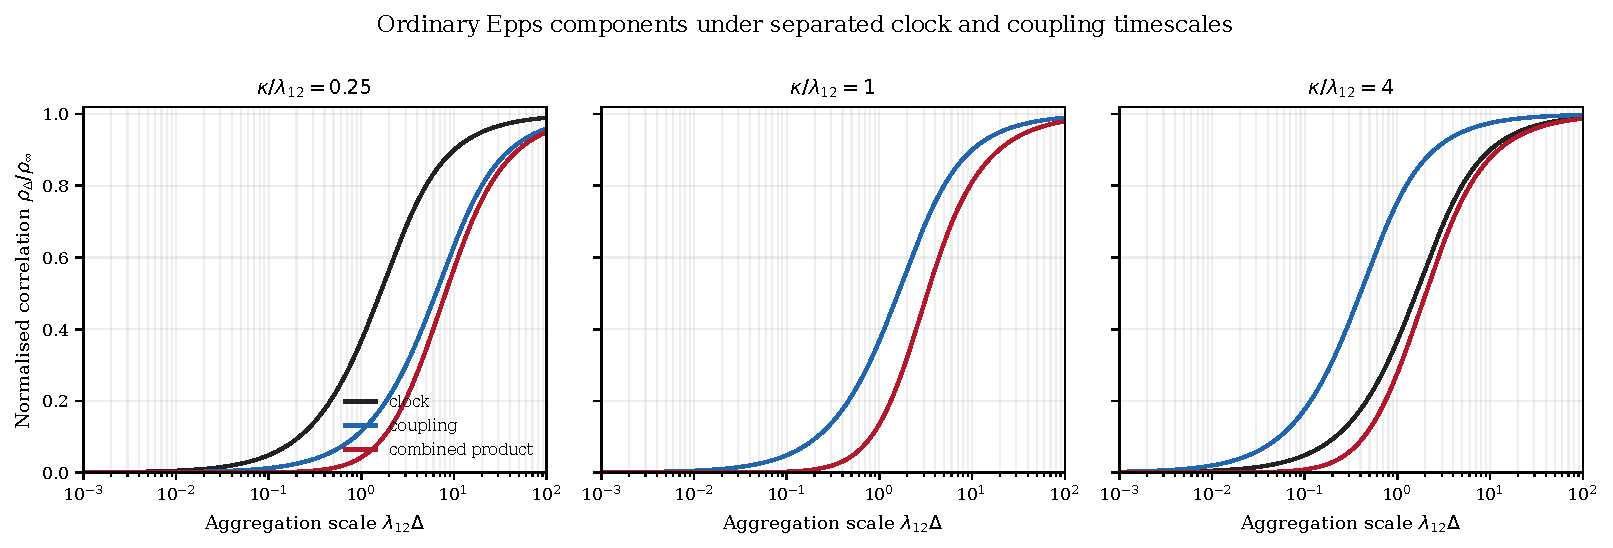
\includegraphics[width=\textwidth]{figures/figure-01-ordinary-epps-components-v1.pdf}
\caption{\textbf{Ordinary Epps components under separated clock and coupling timescales.} The clock curve is $F(\lambda_{12}\Delta)$, the coupling-response curve is $F(\kappa\Delta)$, and the combined curve is their separable product. The horizontal axis is aggregation scale in clock characteristic-time units and the vertical axis is $\rho_\Delta/\rho_\infty$. Panels use $\kappa/\lambda_{12}=0.25,1,4$, with $\lambda_{12}=1$ and $\rho_\infty=1$. The figure shows how the mechanisms contribute across separated and comparable timescales and supplies the analytic component baseline. It supports the component decomposition under the paper's renewal-envelope and separability assumptions; it does not fit market data, simulate an order book, prove statistical independence, or establish the approximation outside those assumptions.}
\label{fig:ordinary-components}
\end{figure}

The short-scale limit of each component is linear in its dimensionless argument, so its rate elasticity approaches one. Once the component reaches its plateau, the elasticity approaches zero. For the product, the partial log-sensitivity to each rate is inherited from that component, while a common proportional perturbation of both rates has the sum of the two partial elasticities.

\begin{figure}[p]
\centering
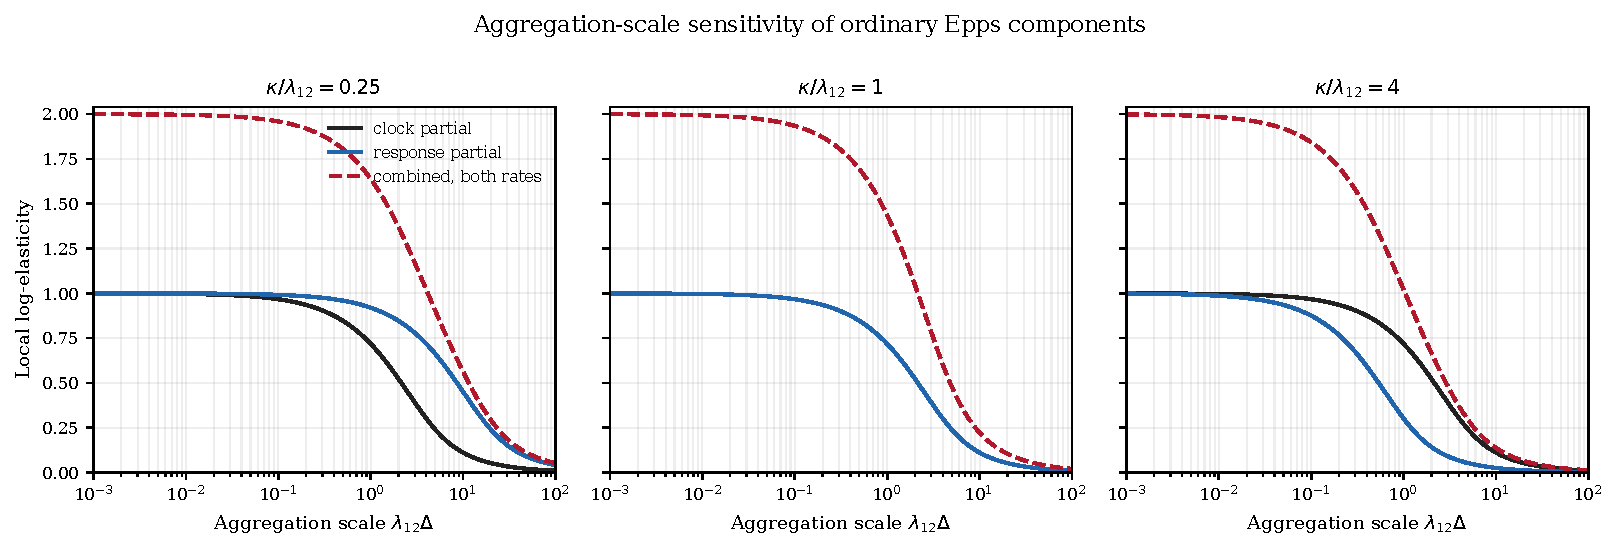
\includegraphics[width=\textwidth]{figures/figure-02-ordinary-epps-sensitivity-v1.pdf}
\caption{\textbf{Aggregation-scale sensitivity of ordinary Epps components.} Curves report $S_F(x)=xF'(x)/F(x)$ for clock refresh and coupling response. The dashed red curve is the log-sensitivity of the combined product when both rates receive the same proportional perturbation. Panels use the Figure~\ref{fig:ordinary-components} rate ratios. Sensitivity tends to one per component in the resolved short-scale limit and to zero on the long-scale plateau, locating the aggregation range that contains rate information. The figure supports local, model-conditional sensitivity statements; it is not a global-identifiability proof, an empirical uncertainty estimate, or evidence that either rate can be recovered without adequate short-scale observations.}
\label{fig:ordinary-sensitivity}
\end{figure}

The combined ordinary curve is invariant under exchange of the clock and response rates. Moreover,
\begin{equation}
C_{\mathrm{combined}}(\Delta)
=\frac{\lambda_{12}\kappa}{4}\Delta^2+O(\Delta^3)
\end{equation}
at short scale. Thus the leading combined curve alone reveals the rate product rather than assigning each timescale to its mechanism. The simulation results below therefore retain independently declared refresh and response rates.

\section{Fractional order sensitivity}

From Eq.~\eqref{eq:fractional},
\begin{equation}
F_\alpha(\Delta;\tau)
=\frac{(\Delta/\tau)^\alpha}{\Gamma(\alpha+2)}
+O(\Delta^{2\alpha}).
\end{equation}
A combined fractional curve therefore has leading power \(\Delta^{\alpha_c+\alpha_r}\). Equal-sum order pairs are deliberately included in Figure~\ref{fig:fractional} to show the resulting local confounding.

\begin{figure}[p]
\centering
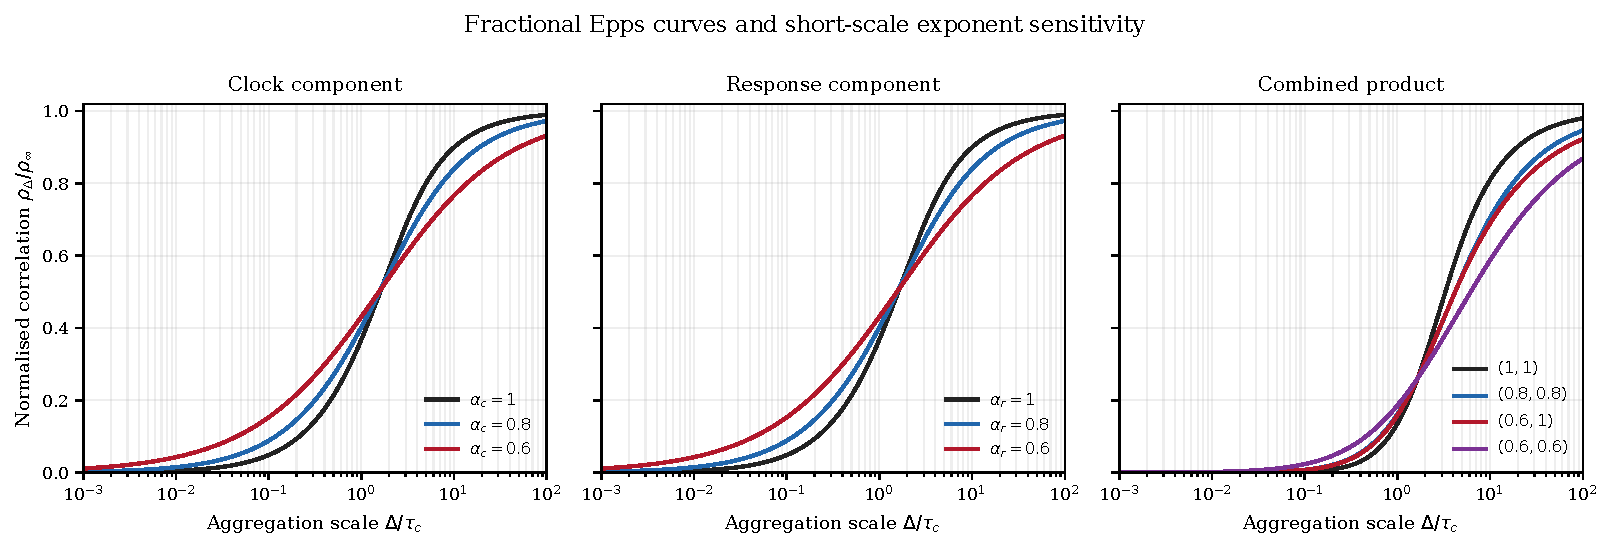
\includegraphics[width=\textwidth]{figures/figure-03-fractional-epps-sensitivity-v1.pdf}
\caption{\textbf{Fractional Epps curves and short-scale exponent sensitivity.} Clock and response components use Eq.~\eqref{eq:fractional}, with unit characteristic times and the diagnosed evaluator recorded in the numerical-design note; \(\alpha=1\) recovers the ordinary kernel. Combined curves use order pairs \((1,1),(0.8,0.8),(0.6,1),(0.6,0.6)\). The equal-sum cases \((0.8,0.8)\) and \((0.6,1)\) share leading short-scale power \(\Delta^{1.6}\), exposing local confounding even when later-scale curvature differs. The figure shows formula sensitivity to fractional order and the ordinary limit. It does not identify both orders from a combined curve alone, attach an unconditional ``slower'' interpretation across dimensional conventions, or validate a fractional market-clock mechanism empirically.}
\label{fig:fractional}
\end{figure}

\section{Conditional reaction-boundary propagation}

Equation~\eqref{eq:response} yields conditional log-elasticities $+1,+1,-1/2,-1$ with respect to coupling strength, source amplitude, source width, and front-slope magnitude. Figure~\ref{fig:boundary} changes one quantity at a time. This is a propagation experiment: multiple structural parameter combinations generate the same effective response rate and hence the same analytic Epps curve.

\begin{figure}[p]
\centering
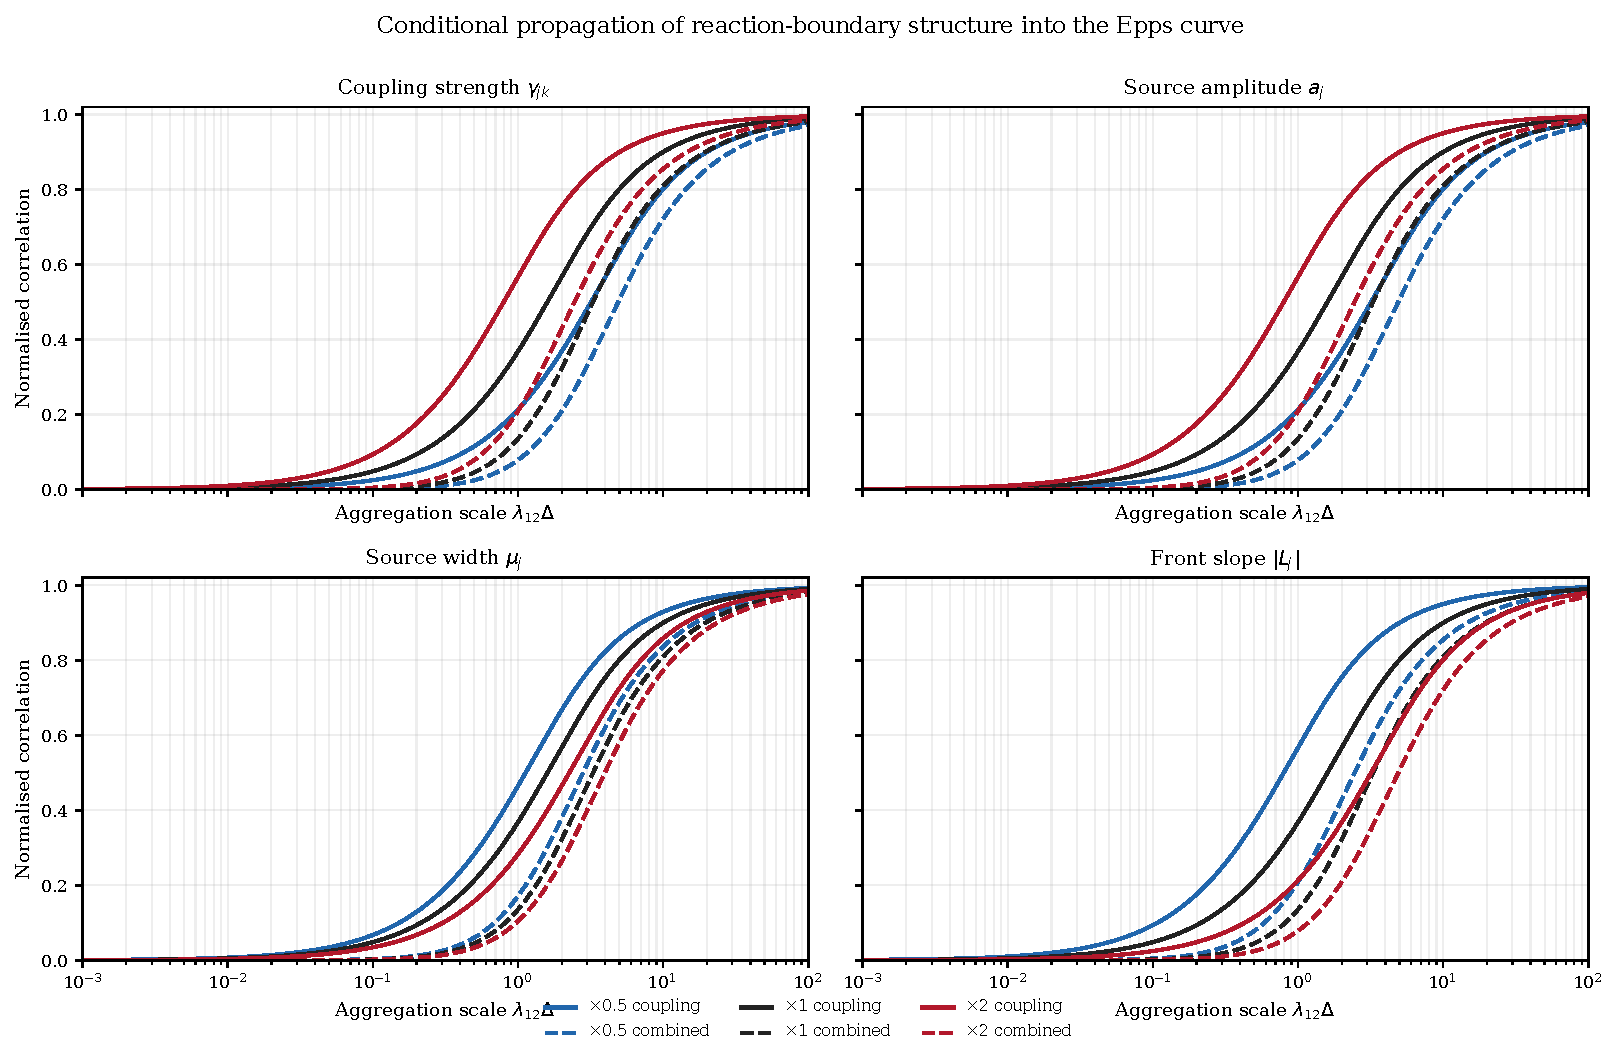
\includegraphics[width=\textwidth,height=0.72\textheight,keepaspectratio]{figures/figure-04-boundary-to-epps-propagation-v1.pdf}
\caption{\textbf{Conditional propagation of reaction-boundary structure into the Epps curve.} The response rate is varied through Eqs.~\eqref{eq:moment}--\eqref{eq:response}. Two symmetric books, unit source amplitude, width and front-slope magnitude, and $\gamma_{jk}=2/\sqrt\pi$ give baseline total response rate $\kappa=1$. Each panel changes one input by factors $0.5,1,2$, holding the others and the unit clock rate fixed; solid curves are coupling factors and dashed curves their combined products with the clock factor. This supports conditional propagation through the analytic response mapping. It does not uniquely infer reaction-front thickness, source width, or coupling strength from an Epps curve and does not claim pointwise equivalence to the legacy lattice coupling.}
\label{fig:boundary}
\end{figure}

Three distinct notions must not be collapsed into a single ``boundary thickness'': the local reaction-front slope \(|\mathcal L_j|\), the continuum selector regularisation \(\varepsilon\), and the lattice spacing \(\Delta x\). The first enters the structural response mapping. The second regularises side selection. The third is a numerical resolution parameter.

\section{Continuum selector and finite-grid representation}

The paper's smooth selector is
\begin{equation}
W(y,z;\varepsilon)=\frac12\left[1+\tanh\left(\frac{yz}{\varepsilon}\right)\right].
\end{equation}
For a centred symmetric full domain, \(yq_j(y)\) is even and the hyperbolic-tangent contribution is odd. Consequently the selected first moment is independent of \(\varepsilon\) in the continuum calculation. Finite domains, misaligned numerical selectors, and coarse grids can break this cancellation. Figure~\ref{fig:grid} diagnoses those representation effects and propagates them through an effective response rate.

\begin{figure}[p]
\centering
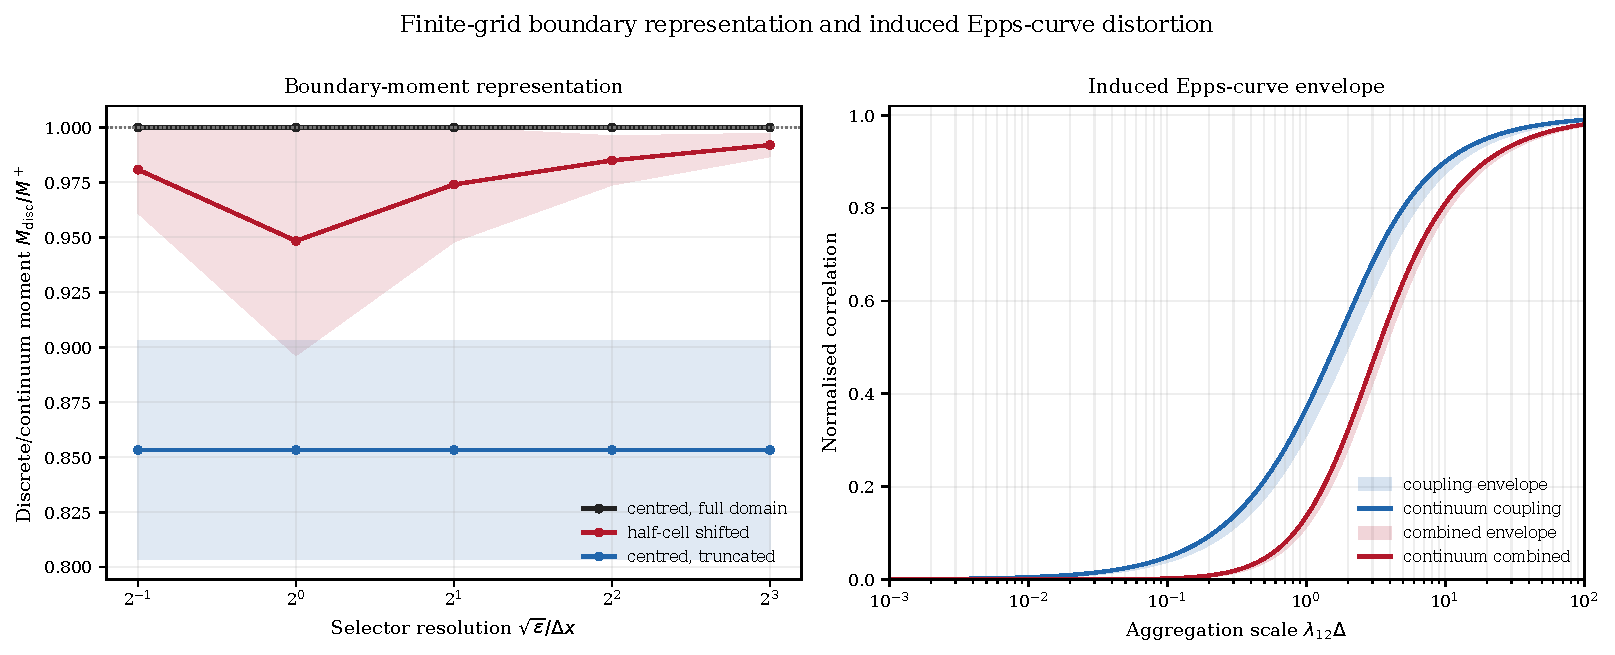
\includegraphics[width=\textwidth]{figures/figure-05-finite-grid-epps-distortion-v1.pdf}
\caption{\textbf{Finite-grid boundary representation and induced Epps-curve distortion.} The left panel reports discrete-to-continuum first-moment ratios as selector resolution \(\sqrt\varepsilon/\Delta x\), lattice spacing, selector alignment, and domain margin vary. Lines give the midpoint and bands the range over four lattice spacings. The centred full-domain case is the parity control; half-cell selector displacement and truncation measure numerical representation errors. The right panel propagates all diagnosed effective-rate ratios through the coupling and combined Epps formulas; lines are continuum baselines and bands are discrete-representation envelopes. Structural parameters are fixed. The figure supports convergence and numerical-sensitivity statements and defines resolution metadata required for v2 overlays. It does not introduce a new continuum Epps mechanism or treat selector width, lattice spacing, and reaction-front thickness as interchangeable.}
\label{fig:grid}
\end{figure}

\clearpage
\section{Calendar-time representation and memory diagnostic}

The aggregation variable in Figures~\ref{fig:ordinary-components}--\ref{fig:grid} remains the observation-window lag, but is reported relative to the clock characteristic time. Writing
\begin{equation}
x=\lambda_{12}\Delta t=\frac{\Delta t}{\tau_c},
\qquad \tau_c=\lambda_{12}^{-1},
\end{equation}
shows that a calendar-time presentation requires only a declared time convention. For an ordinary exponential memory with rate \(r\),
\begin{equation}
h_r(u)=e^{-ru},
\qquad
F(r\Delta t)=1-\frac{1}{\Delta t}\int_0^{\Delta t}h_r(u)\,du.
\label{eq:memory-average}
\end{equation}
For the clock mechanism, \(h_{\lambda_{12}}\) is the no-refresh survival. For the coupling mechanism, \(h_\kappa\) is the relaxation survival and equals the normalised positive-lag exponential covariance kernel used in the paper. Figure~\ref{fig:calendar-bridge} therefore presents the same analytical factors as Figure~\ref{fig:ordinary-components}, not a new Epps mechanism.

\begin{figure}[p]
\centering
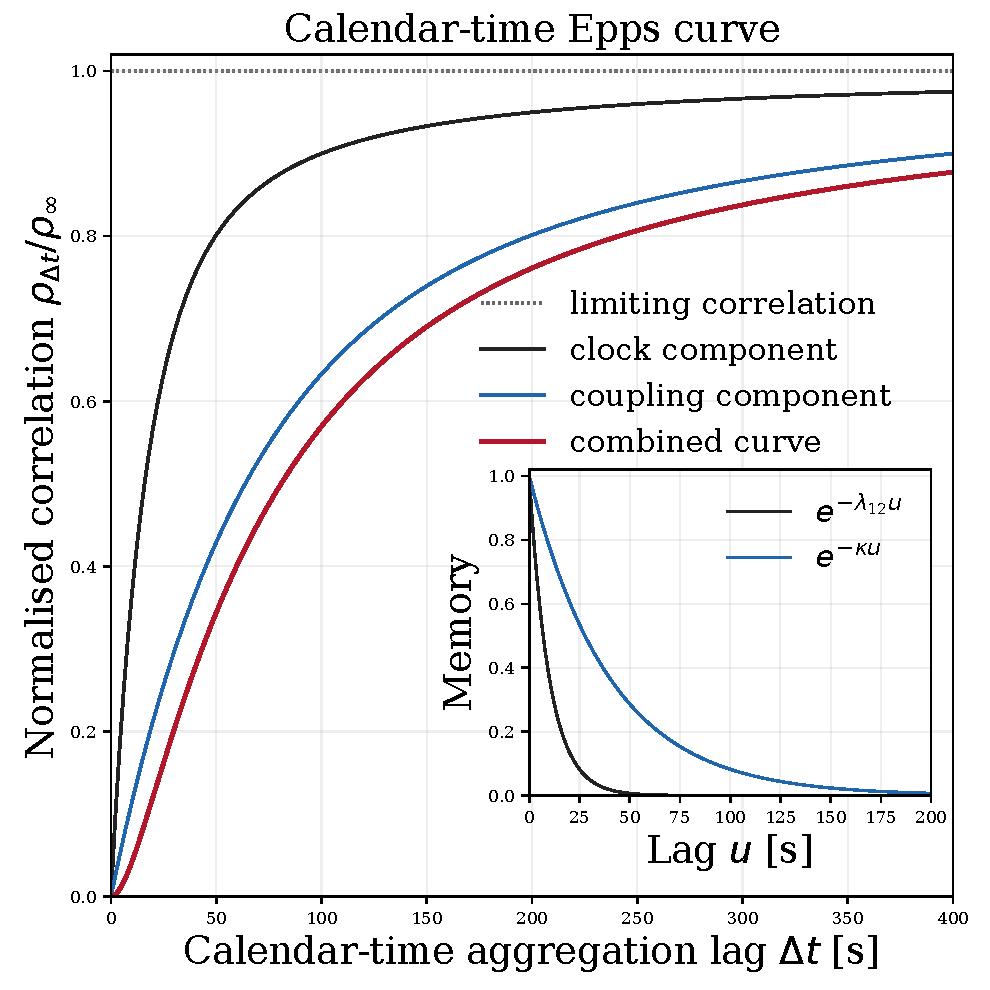
\includegraphics[width=0.91\textwidth]{figures/figure-06-calendar-time-epps-memory-v1.pdf}
\caption{\textbf{Calendar-time Epps curve.} The square main panel rewrites the Figure~\ref{fig:ordinary-components} slow-response profile on a linear calendar-time axis using the explicitly illustrative convention $\lambda_{12}=0.1\,\mathrm{s}^{-1}$, $\kappa=0.025\,\mathrm{s}^{-1}$, and $\rho_\infty=1$, corresponding to $\tau_c=10$ s and $\tau_r=40$ s. Black, blue and red curves are the clock factor, coupling factor and their leading-order separable product; the grey dotted line marks the normalised limiting correlation $\rho_{\Delta t}/\rho_\infty=1$. The enlarged inset reports $h_c(u)=e^{-\lambda_{12}u}$ and $h_r(u)=e^{-\kappa u}$: respectively the no-refresh survival and coupling-relaxation survival, with the latter also equal to the normalised positive-lag exponential covariance kernel. The seconds scale is not fitted to data, and the inset is neither a path autocorrelation nor a power-spectrum estimate. Path-derived autocorrelations are reported separately in Figure~\ref{fig:dependence}.}
\label{fig:calendar-bridge}
\end{figure}

The distinction from the simulation output is substantive. A sample autocorrelation requires a generated path, a declared estimator and finite-sample uncertainty. The deterministic inset exposes only the memory functions that enter Eq.~\eqref{eq:memory-average}. Figure~\ref{fig:dependence} reports the separate path-derived log-mid increment and trade-sign autocorrelations without retrospectively relabelling this analytical diagnostic.

\clearpage
\section{Uniform-operational simulation}

Let \(u_n=n\Delta u\) be the common operational grid. Both density fields are
advanced on this grid before any calendar observation is constructed. External
innovations are book-specific, the translation-mode coupling uses
Eq.~\eqref{eq:translation-mode}, and labelled order events modify the density
state at declared operational steps. The boundary price is the accepted unique
interior zero crossing of the signed density field.

For book \(j\), let \(\tau_{j,m}\) be its completed calendar refresh events.
The software first selects the latest event at or before \(t\), then the latest
uniform operational node at or before that event:
\begin{equation}
m_j(t)=\max\{m:\tau_{j,m}\leq t\},
\qquad
n_j(t)=\max\{n:u_n\leq\tau_{j,m_j(t)}\},
\qquad
P_j^{\rm cal}(t)=P_j^{\rm op}(u_{n_j(t)}).
\label{eq:subordination}
\end{equation}
Equation~\eqref{eq:subordination} is previous-refresh subordination. It selects
an already completed state and never changes an operational update interval.

\input{source/source-v2/NUMERICAL-ALGORITHMS-v2.2.0.tex}

\subsection{Theory-to-simulation Epps comparison}

Figure 7 in this supplement corresponds to Figure 1 in the paper. Its combined three-square layout retains common axis limits and component colours; separate square exports are also supplied. Each comparison uses 512 independent validation paths, 8000 seconds after 200 seconds of dynamical warm-up, $\Delta x=0.1$ and a 0.5-second update. The clock-only and combined panels use four book-specific Poisson-clock replicates per path. A replicate is not an additional independent operational path. The existing 256-path independent calibration ensembles remain available as diagnostics.

The normalization is explicit. In Figure 7a the plotted attenuation is the ratio of asynchronous to synchronous pooled return correlations on the \emph{same} validation ensemble:
\begin{equation}
\widehat A(\Delta)=\frac{\widehat\rho_{\mathrm{async}}(\Delta)}
{\widehat\rho_{\mathrm{sync}}(\Delta)}.
\label{eq:matched-clock}
\end{equation}
In Figures 7b and 7c let $X=(P_1+P_2)/2$. The plotted normalized covariance is
\begin{equation}
\widehat B_c(\Delta)=
\frac{\sum_{g,r}\overline{R^{(c)}_{1,g,r}R^{(c)}_{2,g,r}}}
{\sum_{g,r}(R^{\mathrm{op}}_{X,g,r})^2},
\label{eq:matched-covariance}
\end{equation}
where $g$ denotes an independent path, $r$ an admissible origin, and the overbar averages clock replicates where applicable. It is a covariance response, not Pearson correlation. These matched estimators differ from dividing by an independently estimated long-scale covariance rate times $\Delta$ in the published comparison. Matching retains numerator--denominator dependence and reduces normalization noise; it is not a fit of a response rate or a time map.

Shading in all three panels is the approximate pointwise 98\% interval
$\widehat\theta\pm t_{0.99,511}\operatorname{se}_{\mathrm{JK}}(\widehat\theta)$,
using a delete-one-independent-path jackknife that recomputes the complete ratio. The critical multiplier is approximately 2.334. These intervals describe uncertainty in the estimated mean/pooled statistic, not the spread of individual paths, simultaneous coverage over all lags, or discretization/model error. The increase from 95\% to 98\% widens them by about 19\%; there is no minimum graphical width. A narrow band may remain largely hidden by coincident curves at the printed scale. Black reference strokes are wider than the coloured simulation strokes so that both remain noticeable at overlap.

The black clock curve is the equal-rate previous-refresh factor. The black combined curve remains the paper's product approximation. The dashed grey curve is the stationary joint reduced reference in Eq.~\eqref{eq:joint-poisson-coupling}. The reduced conditional moments at the realized refresh indices are retained in the supplied numerical comparison; neither reference is an exact identity for the full reaction--diffusion dynamics. No smoothing of simulated means, selected-seed replacement, or parameter refitting is applied.

\paragraph{Why the combined curve differs from the product.}
Clock-only attenuation and coupling-induced covariance describe different operations. The clock selects observation times; coupling spreads cross-book dependence over time. Applying independent clocks to a coupled process therefore requires averaging that time-dependent covariance over the sampled intervals. It is not equivalent to multiplying the two separately averaged component curves.

This distinction can be calculated explicitly for the stationary reduced model underlying the grey reference. Write $P_1=X+Z/2$ and $P_2=X-Z/2$, with independent Brownian pair centre $X$ and stationary Ornstein--Uhlenbeck spread $Z$. Let $C$ be the variance rate of $X$, and use the spread variance $2C/\kappa$ of the symmetric closure. The cross-covariance kernel of price increments is
\begin{equation}
K_{12}(s)=\frac{C\kappa}{2}e^{-\kappa|s|}.
\end{equation}
For independent stationary Poisson observation clocks, each of rate $\lambda=\lambda^{\rm clk}$ and independent of the prices, previous-refresh observation convolves this cross-kernel with the difference-of-clock-age density $h_\lambda(s)=(\lambda/2)e^{-\lambda|s|}$. This is a cross-book result; it does not apply the same convolution to a book's marginal variance. Integrating the resulting kernel over a return window gives
\begin{align}
G(\Delta)
&=\frac{2}{C\Delta}\int_0^\Delta(\Delta-s)
       (K_{12}*h_\lambda)(s)\,ds \\
&=\frac{\lambda^2F(\kappa\Delta)-\kappa^2F(\lambda\Delta)}
        {\lambda^2-\kappa^2},\qquad \lambda\ne\kappa.
\label{eq:joint-poisson-coupling}
\end{align}
At equal rates the continuous limit is $G(\Delta)=F(x)-xF'(x)/2$, with $x=\kappa\Delta$. Equation~\eqref{eq:joint-poisson-coupling} is a population covariance normalized by $C\Delta$. It is the stationary continuous-time counterpart of the reduced conditional calculation, not an exact solution of the full reaction--diffusion dynamics or a finite-sample ratio identity.

The short-time powers expose the difference:
\begin{equation}
G(\Delta)=\frac{\lambda\kappa}{2(\lambda+\kappa)}\Delta+O(\Delta^3),
\qquad
F(\lambda\Delta)F(\kappa\Delta)
=\frac{\lambda\kappa}{4}\Delta^2+O(\Delta^3).
\label{eq:joint-short-time}
\end{equation}
The joint reduced response starts linearly, whereas the product starts quadratically. Thus the paper's product approximation is not the short-time asymptotic of this joint reduced model. With the fixed rates $\lambda=0.1$ and $\kappa=0.025\,\mathrm{s}^{-1}$, at 20 seconds the joint expression is 0.18942, the product is 0.12095, and the pooled simulation is 0.18717. Increasing the ensemble can expose this approximation residual more clearly, but cannot remove it. Both analytical expressions tend to one as the aggregation lag increases.

The mean clock wait is 10 seconds and the coupling relaxation time is 40 seconds. The earlier Figure 7 curves began at 20 seconds, where the clock factor has already reached 0.568. A log--log change of axes alone cannot recover the missing initial rise. The short-lag extension therefore evaluates all three panels below 20 seconds and checks the numerical grid separately from sampling precision. The algebra above was checked against direct kernel convolution and return-window quadrature without parameter fitting.

\paragraph{Short-lag numerical check.}
The same 512-path ensembles were replayed at eight additional lags: 0.5, 1, 2, 3, 5, 7.5, 10 and 15 seconds. Their previously saved moments at 20--400 seconds were recovered before the additional lags were used. At 0.5 seconds, the clock-only estimate is $0.02460\pm0.00064$, compared with $F(0.05)=0.02459$, and the combined estimate is $0.00531\pm0.00075$, compared with $G(0.5)=0.00500$; the quoted uncertainties are pointwise 98\% half-widths.

The coupling-only value at that lag is $-0.00638\pm0.00167$, compared with the continuous reduced value 0.00622. Here the return contains only one 0.5-second update. The explicit discrete reduced closure explains why this distinction matters. With update $h$, spread coefficient $q=1-\kappa h$ and $\Delta=mh$, its stationary normalized synchronous covariance is
\begin{equation}
B_h(\Delta)=1-\frac{1-(1-\kappa h)^m}
 {\kappa\Delta(1-\kappa h/2)},\qquad 0<\kappa h<2.
\label{eq:discrete-coupling}
\end{equation}
At one update, $B_h(h)=-\kappa h/(2-\kappa h)$, which is $-0.00629$ here. The two coupling drifts oppose one another, while a new independent shock reaches the other book through subsequent updates. This discrete result is a reduced benchmark, not an exact identity for the full density solver. As $h\to0$ at fixed $\Delta$, it tends to $F(\kappa\Delta)$.

A paired 64-path, 2000-second screen compared $(\Delta x,h)=(0.1,0.5\,\mathrm{s})$ and $(0.05,0.125\,\mathrm{s})$, preserving the diffusion scaling and using nested innovations and the same continuous observation clocks. At the 0.5-second lag the coupling-only change is $+0.00938\pm0.00009$; the clock-only and combined changes are $-0.00047\pm0.00091$ and $+0.00001\pm0.00113$. Thus sampling precision, discrete updating and product approximation have different roles. The main figure retains the declared 512-path production grid, and the paired refinement results are summarized above. The smallest-lag coupling-only points are not continuum-converged; the required scale ordering is $h\ll\Delta$. Nonpositive estimates and interval endpoints remain visible on the linear axes and are omitted from the log--log axes.


\paragraph{Comparison with the published Figure 7.}
The v2.1.0 shading represents pointwise 95\% jackknife uncertainty in the estimated simulation statistic, not the distribution of individual sample paths. In panel (c), the covariance was divided by a frozen, independently calibrated covariance rate times the aggregation lag. The plotted standard errors condition on that frozen rate. The v2.2.0 comparison uses the matched pair-centre denominator in Eq.~\eqref{eq:matched-covariance}, 512 validation paths and longer records, retaining numerator--denominator dependence. Consequently the change in envelope width cannot be attributed to path count alone.

Across the 20 common lags from 20 to 400 seconds, the old combined 95\% interval has maximum half-width 0.19958; the new matched 98\% interval has maximum half-width 0.00717. Recomputing the new ensemble with independent calibration held fixed gives maximum 98\% half-width 0.02807, while changing the mean by at most 0.00151 relative to the matched estimator. This isolates a substantial normalization contribution to precision on the same new ensemble; it does not measure uncertainty in the calibration rate itself.

The black leading-order product is inside the published 95\% intervals at 18 of 20 lags, whereas the grey same-clock conditional reference is inside at all 20. At $\Delta=20$ s, the published simulation is 0.20416, the product is 0.12095, and the interval half-width is 0.03423: even the published band excludes the product there. In the new comparison the product is outside the 98\% intervals at all 20 lags, while the conditional reference remains inside all 20. These are descriptive counts across correlated lags, not simultaneous coverage tests. The increased precision exposes the distinction between a product of component factors and the conditional calculation using the actual refresh indices. It does not establish an exact identity between the reduced reference and full reaction--diffusion dynamics. Enlarging the ensemble cannot remove a systematic approximation residual.

\setcounter{figure}{6}
\begin{figure}[p]
\centering
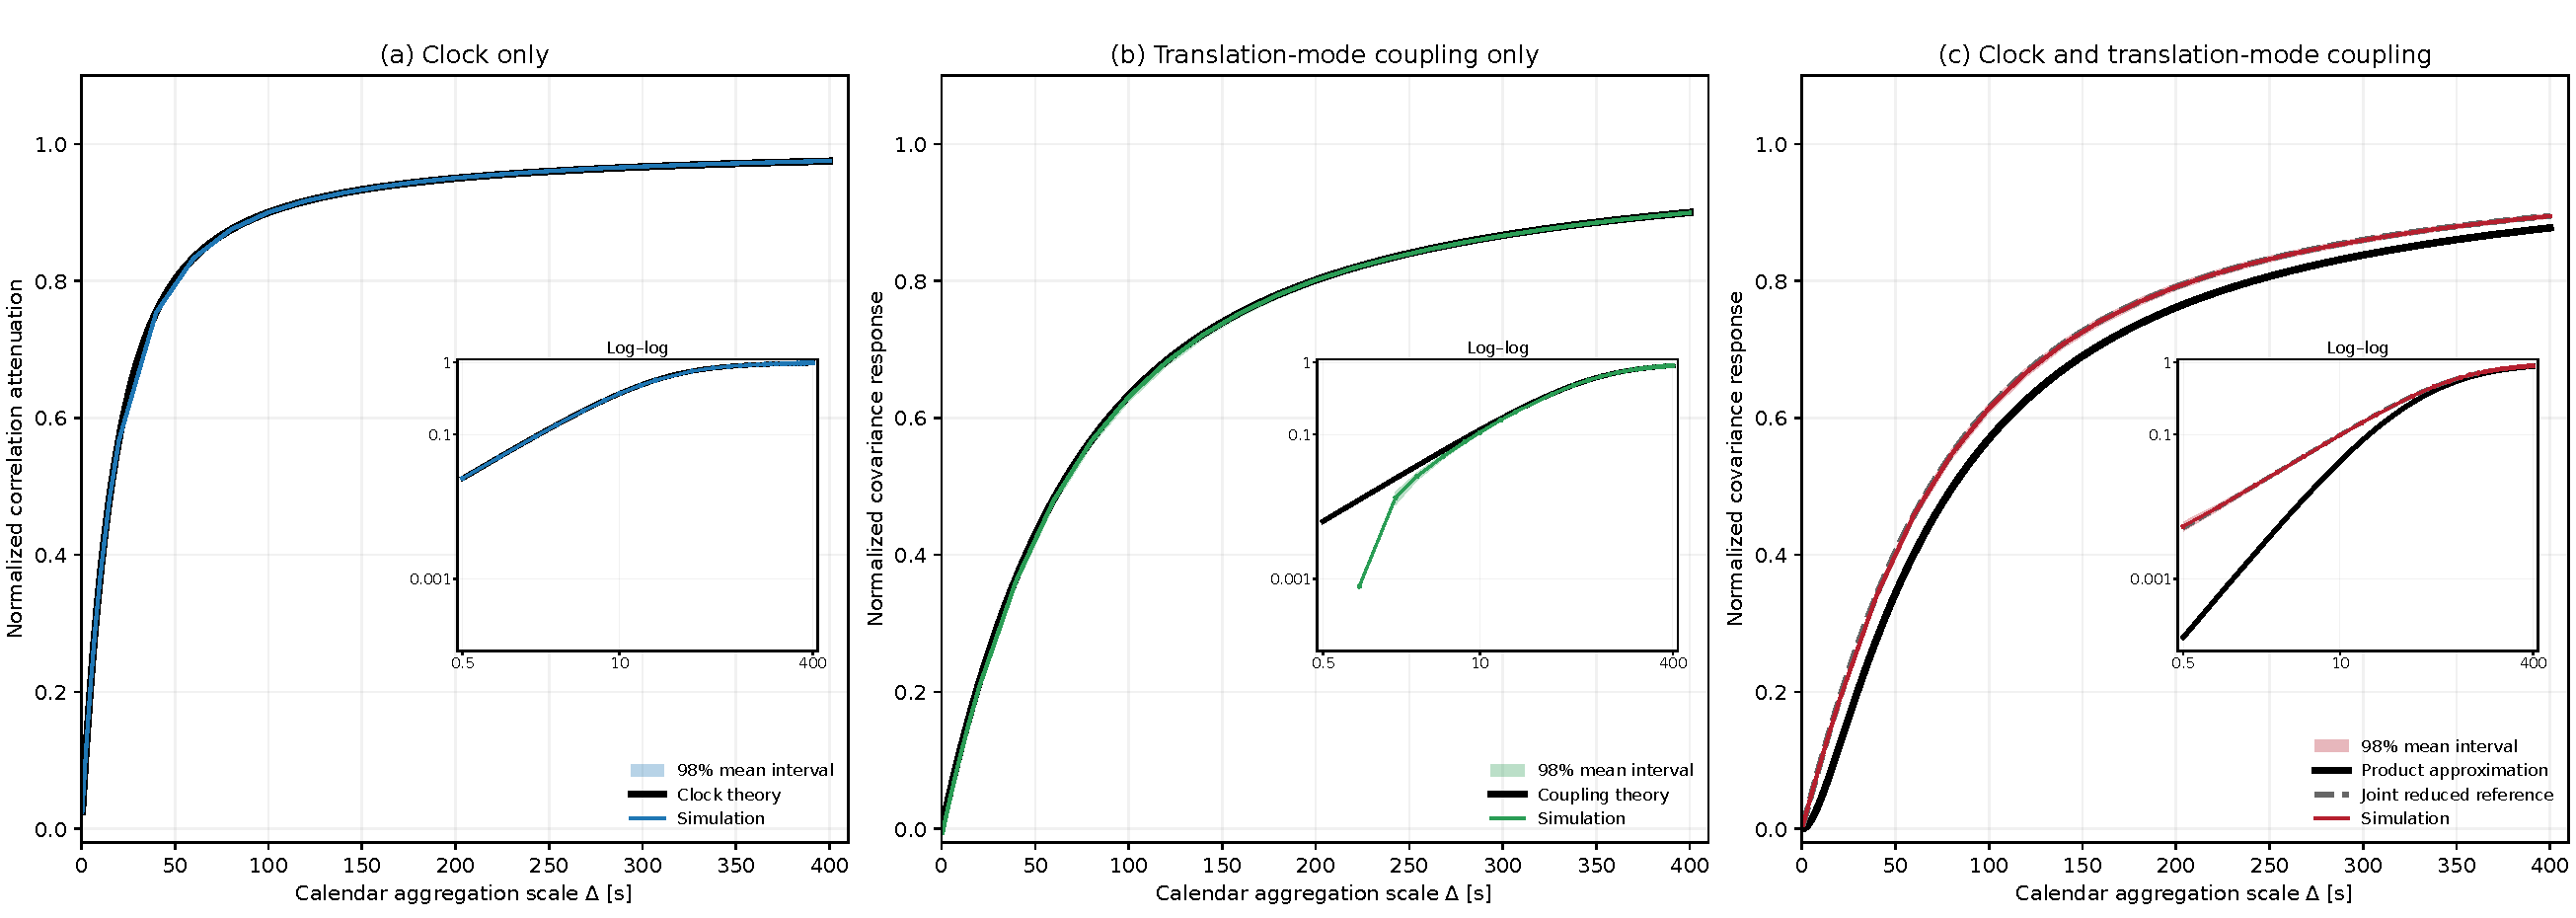
\includegraphics[width=\textwidth]{figures/figure-07-final-estimator-aware-epps-v2.pdf}
\caption{\textbf{Clock and translation-mode Epps comparisons.} Three square panels share aggregation scales and vertical limits. (a) Blue: matched clock attenuation; black: equal-rate clock factor, with each book's rate $0.1\,\mathrm{s}^{-1}$. (b) Green: matched coupling covariance; black: coupling factor with $\kappa=0.025\,\mathrm{s}^{-1}$. (c) Red: matched combined covariance; black: product approximation; dashed grey: stationary joint reduced reference $G(\Delta)$ in Eq.~\eqref{eq:joint-poisson-coupling}. Shading denotes approximate pointwise 98\% mean intervals across 512 independent paths, grouping four clock replicates per path where applicable. Maximum half-widths are 0.00217, 0.00749 and 0.00717 respectively. The narrow band in (c) resolves the product-approximation difference; it is not an individual-path envelope. No parameters are refitted. Insets repeat the curves and intervals on log--log axes over the measured 0.5--400 s range. The smallest-lag coupling-only points remain sensitive to the update size; nonpositive values are shown only on the linear axes. Separate square exports accompany this combined figure.}
\label{fig:final-epps}
\end{figure}
\makeatletter
\def\@currentlabel{7a}\label{fig:final-epps-clock}
\def\@currentlabel{7b}\label{fig:final-epps-coupling}
\def\@currentlabel{7c}\label{fig:final-epps-combined}
\makeatother

\subsection{Translation-mode component}

The translation-mode coupling is tested separately under identity clocks before it is
used in the combined route. Deterministic signed-front relaxations diagnose the
registered response rate; stochastic holdout paths test normalized covariance
and the distinct finite-scale return correlation. The covariance scale is
frozen from a disjoint calibration ensemble.

\begin{figure}[p]
\centering
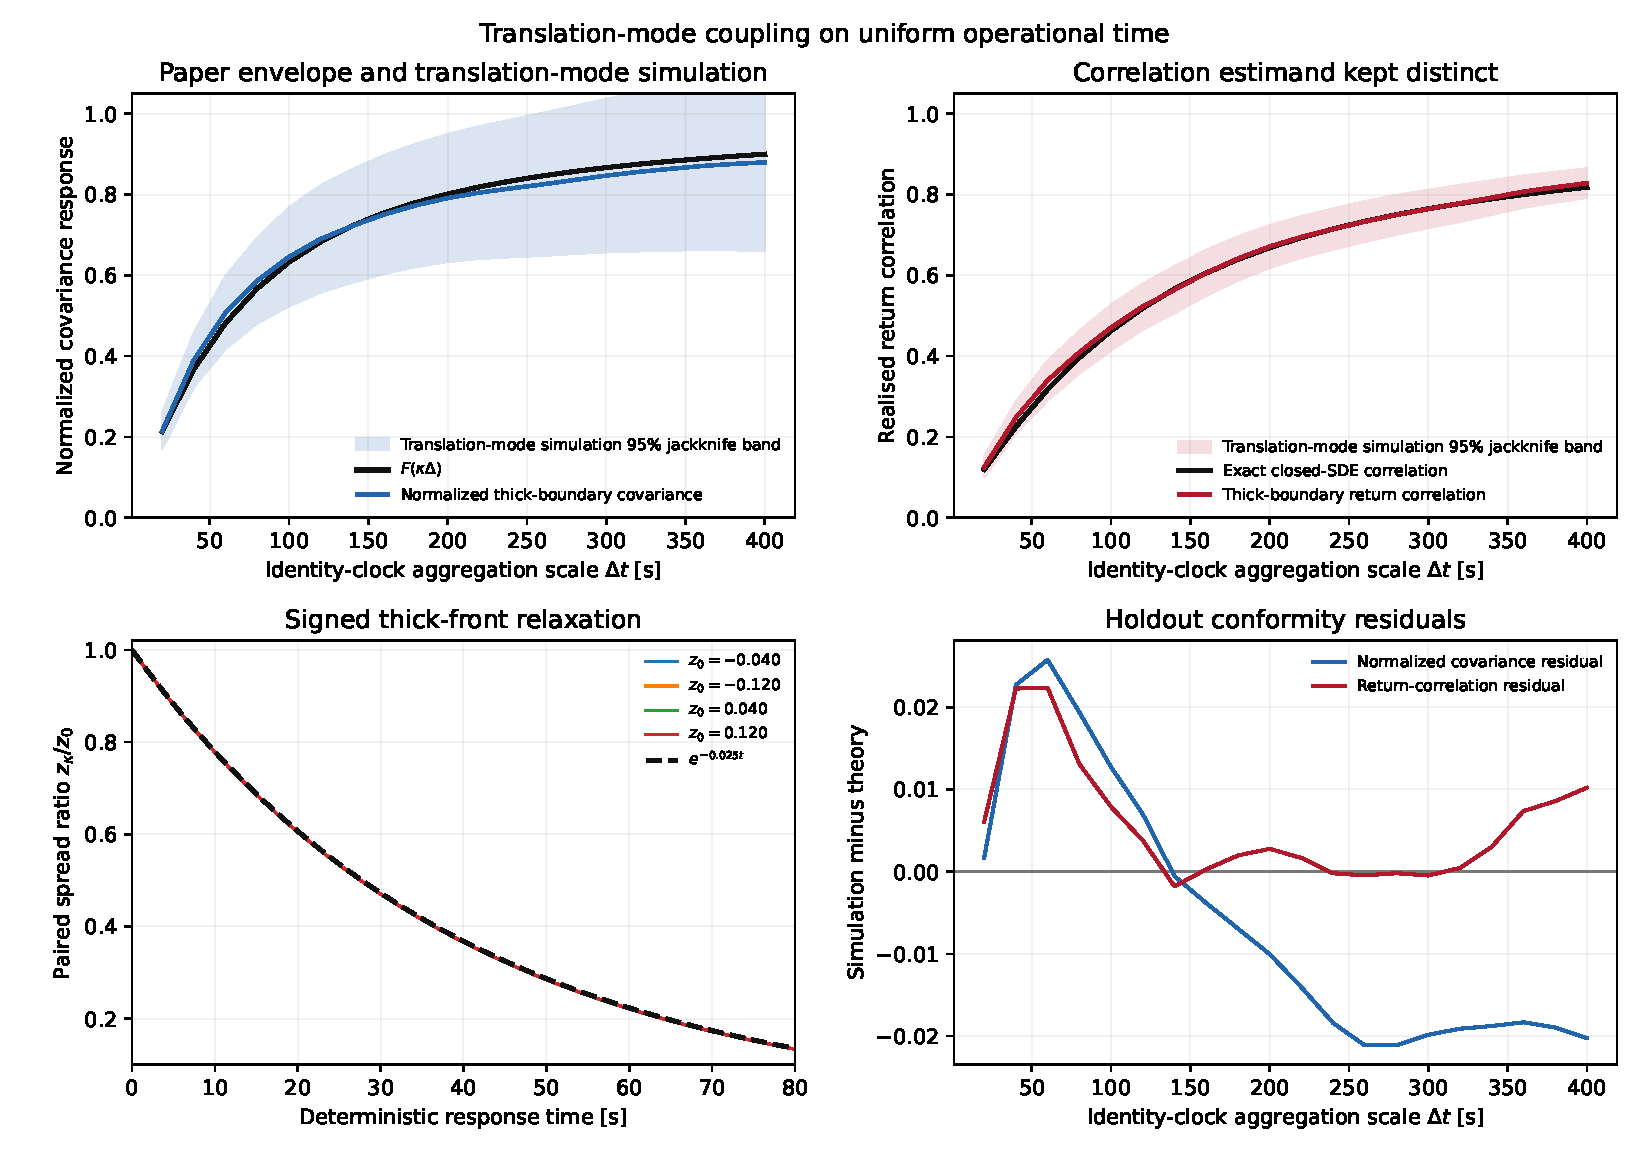
\includegraphics[width=\textwidth]{figures/figure-08-corrected-translation-mode-coupling-v2.pdf}
\caption{\textbf{Translation-mode coupling on uniform operational time.} Retained v2.1.0 component diagnostic. Holdout thick-boundary paths are compared with the analytical normalized covariance response and the distinct finite-scale return correlation. The covariance rate is estimated on a disjoint calibration ensemble, as in the published diagnostic. Lower panels verify signed deterministic front relaxation and residuals at the frozen response rate. No clock, interpolation or parameter fit enters this comparison.}
\label{fig:translation-mode-coupling}
\end{figure}

\section{Event impact and dependence diagnostics}

Market-order events consume opposing density at the active boundary and are
recorded on an immutable event tape. Impact is measured by pairing each event
path with an otherwise identical zero-input control. Responses are
aggressor-signed log-boundary differences, so own and cross effects use one
common linear scale. Calendar versions are obtained only after the operational
paths are complete, using Eq.~\eqref{eq:subordination}.

\begin{figure}[p]
\centering
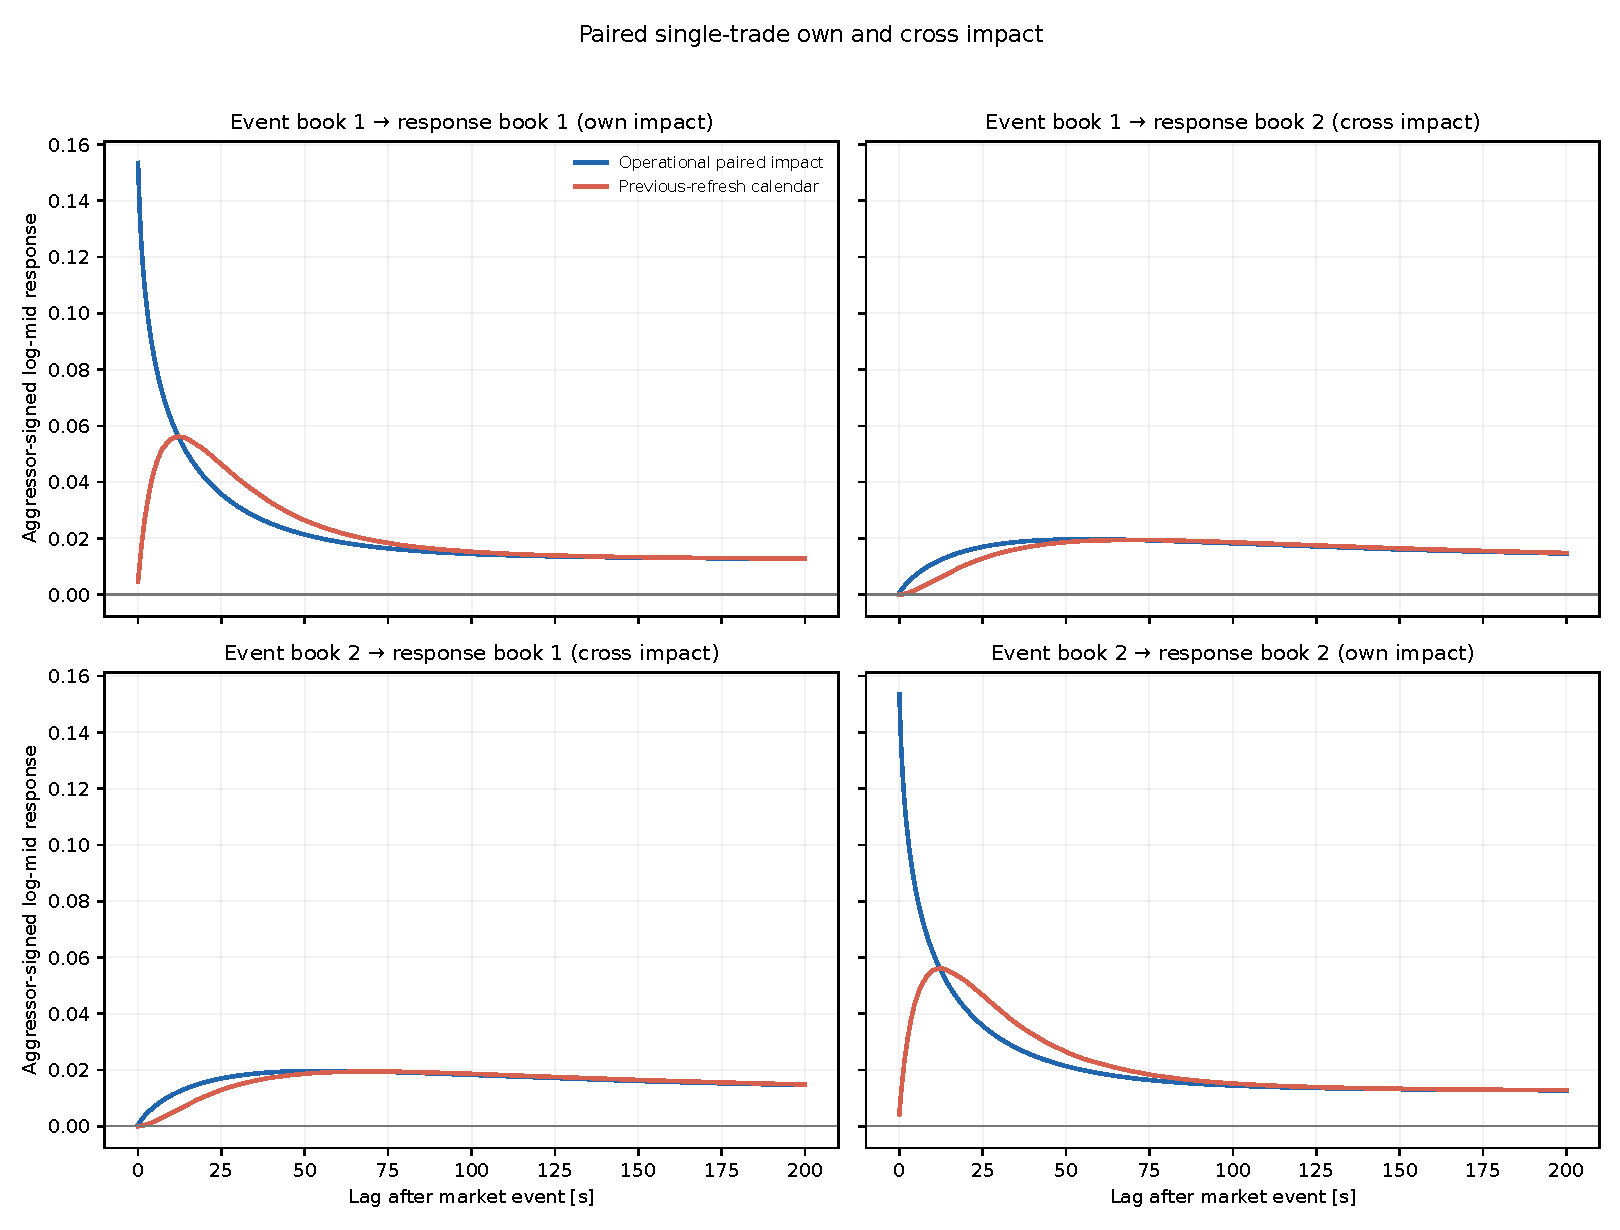
\includegraphics[width=\textwidth]{figures/figure-09-single-trade-impact-v2.pdf}
\caption{\textbf{Paired single-trade own and cross impact.} Rows identify the event book and columns the response book, preserving the full directional matrix on a common linear scale. Blue denotes operational impact; red denotes Poisson previous-refresh impact. Curves average 512 independent primitive groups, with signs, four symmetry partners and four clock replicates grouped before calculating pointwise 95\% mean intervals. The order quantity is 0.05, $\Delta x=0.05$, and the calendar-equivalent update is 0.125 seconds. Physical injection occurs at 150 seconds; displayed lag zero retains the recorded 150.5-second completion anchor. Clock-inactive observations are included. Bands describe sampling uncertainty and do not include spatial discretization error.}
\label{fig:single-trade}
\end{figure}

A meta-order is a declared schedule of child market orders with fixed total
quantity and book. Equal-volume horizon comparisons distinguish schedule timing
from a true participation rate, which would require background market-order
volume not present in this model.

\begin{figure}[p]
\centering
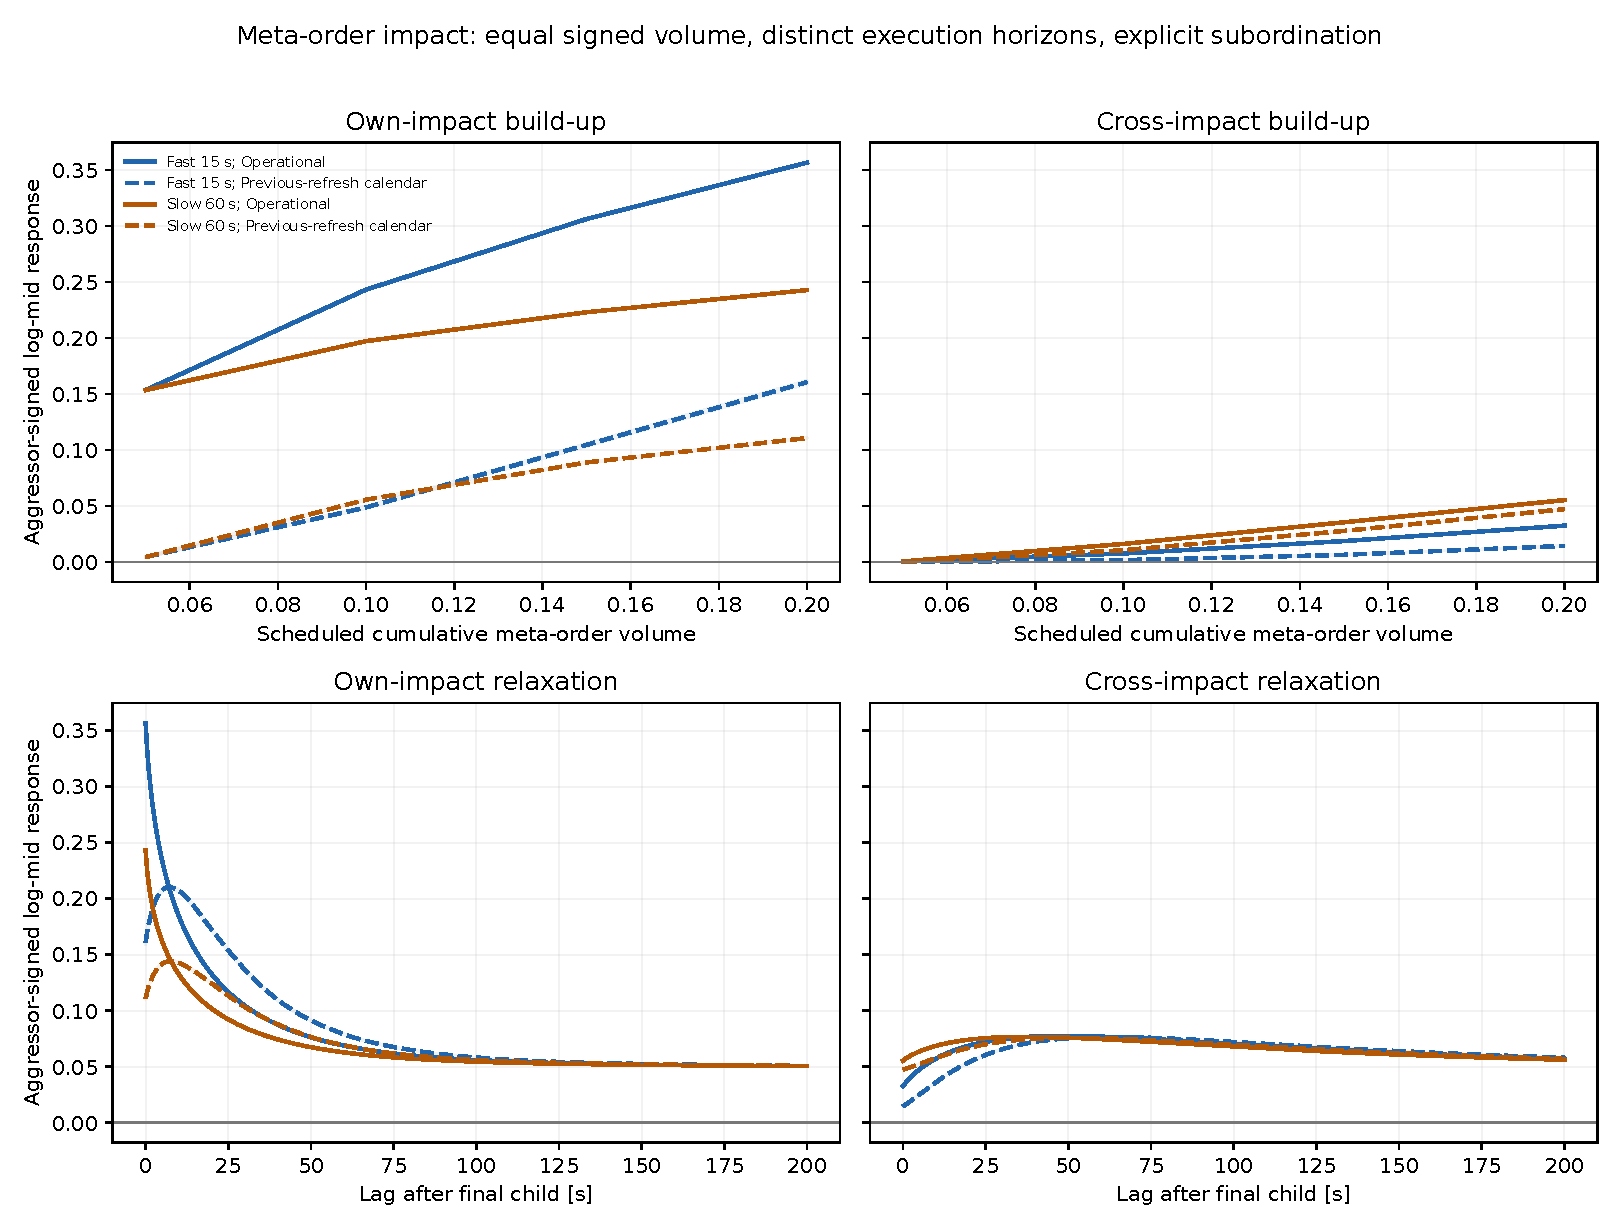
\includegraphics[width=\textwidth]{figures/figure-10-meta-order-impact-v2.pdf}
\caption{\textbf{Scheduled meta-order own and cross impact.} Build-up is above relaxation; own and cross responses occupy the two columns on a shared vertical scale. Blue denotes the fast 15-second schedule and brown the slow 60-second schedule; solid denotes operational observation and dashed Poisson previous refresh. Four children of quantity 0.05 give total signed volume 0.20. Means and pointwise 95\% intervals use 512 independent groups with the grouping and $\Delta x=0.05$ grid of Figure~\ref{fig:single-trade}. Physical injection times are preserved under refinement. Relaxation lag zero is the recorded completion anchor, 0.5 seconds after the final physical injection. Equal volume and distinct execution duration are schedule controls, not estimates of a market participation rate.}
\label{fig:meta-order}
\end{figure}

For a sequence \(X_n\), let \(\bar X_{L,k}\) and \(\bar X_{R,k}\) denote the
separate sample means of \(\{X_n\}_{n=1}^{N-k}\) and
\(\{X_{n+k}\}_{n=1}^{N-k}\).  The registered positive-lag statistic is the
Pearson correlation of those two overlapping slices,
\begin{equation}
\widehat\rho_X(k)=
\frac{\sum_{n=1}^{N-k}\bigl(X_n-\bar X_{L,k}\bigr)
\bigl(X_{n+k}-\bar X_{R,k}\bigr)}
{\sqrt{\left[\sum_{n=1}^{N-k}\bigl(X_n-\bar X_{L,k}\bigr)^2\right]
\left[\sum_{n=1}^{N-k}\bigl(X_{n+k}-\bar X_{R,k}\bigr)^2\right]}},
\qquad \widehat\rho_X(0)=1.
\label{eq:pearson-slice-acf}
\end{equation}
The price statistic is applied to log-mid increments, never to price levels.
Trade-sign diagnostics distinguish ground-truth aggressor signs, a
quote/midpoint rule and the historically inherited tick rule. Event-time signs
and calendar-binned signed flow are separate estimands.

\begin{figure}[p]
\centering
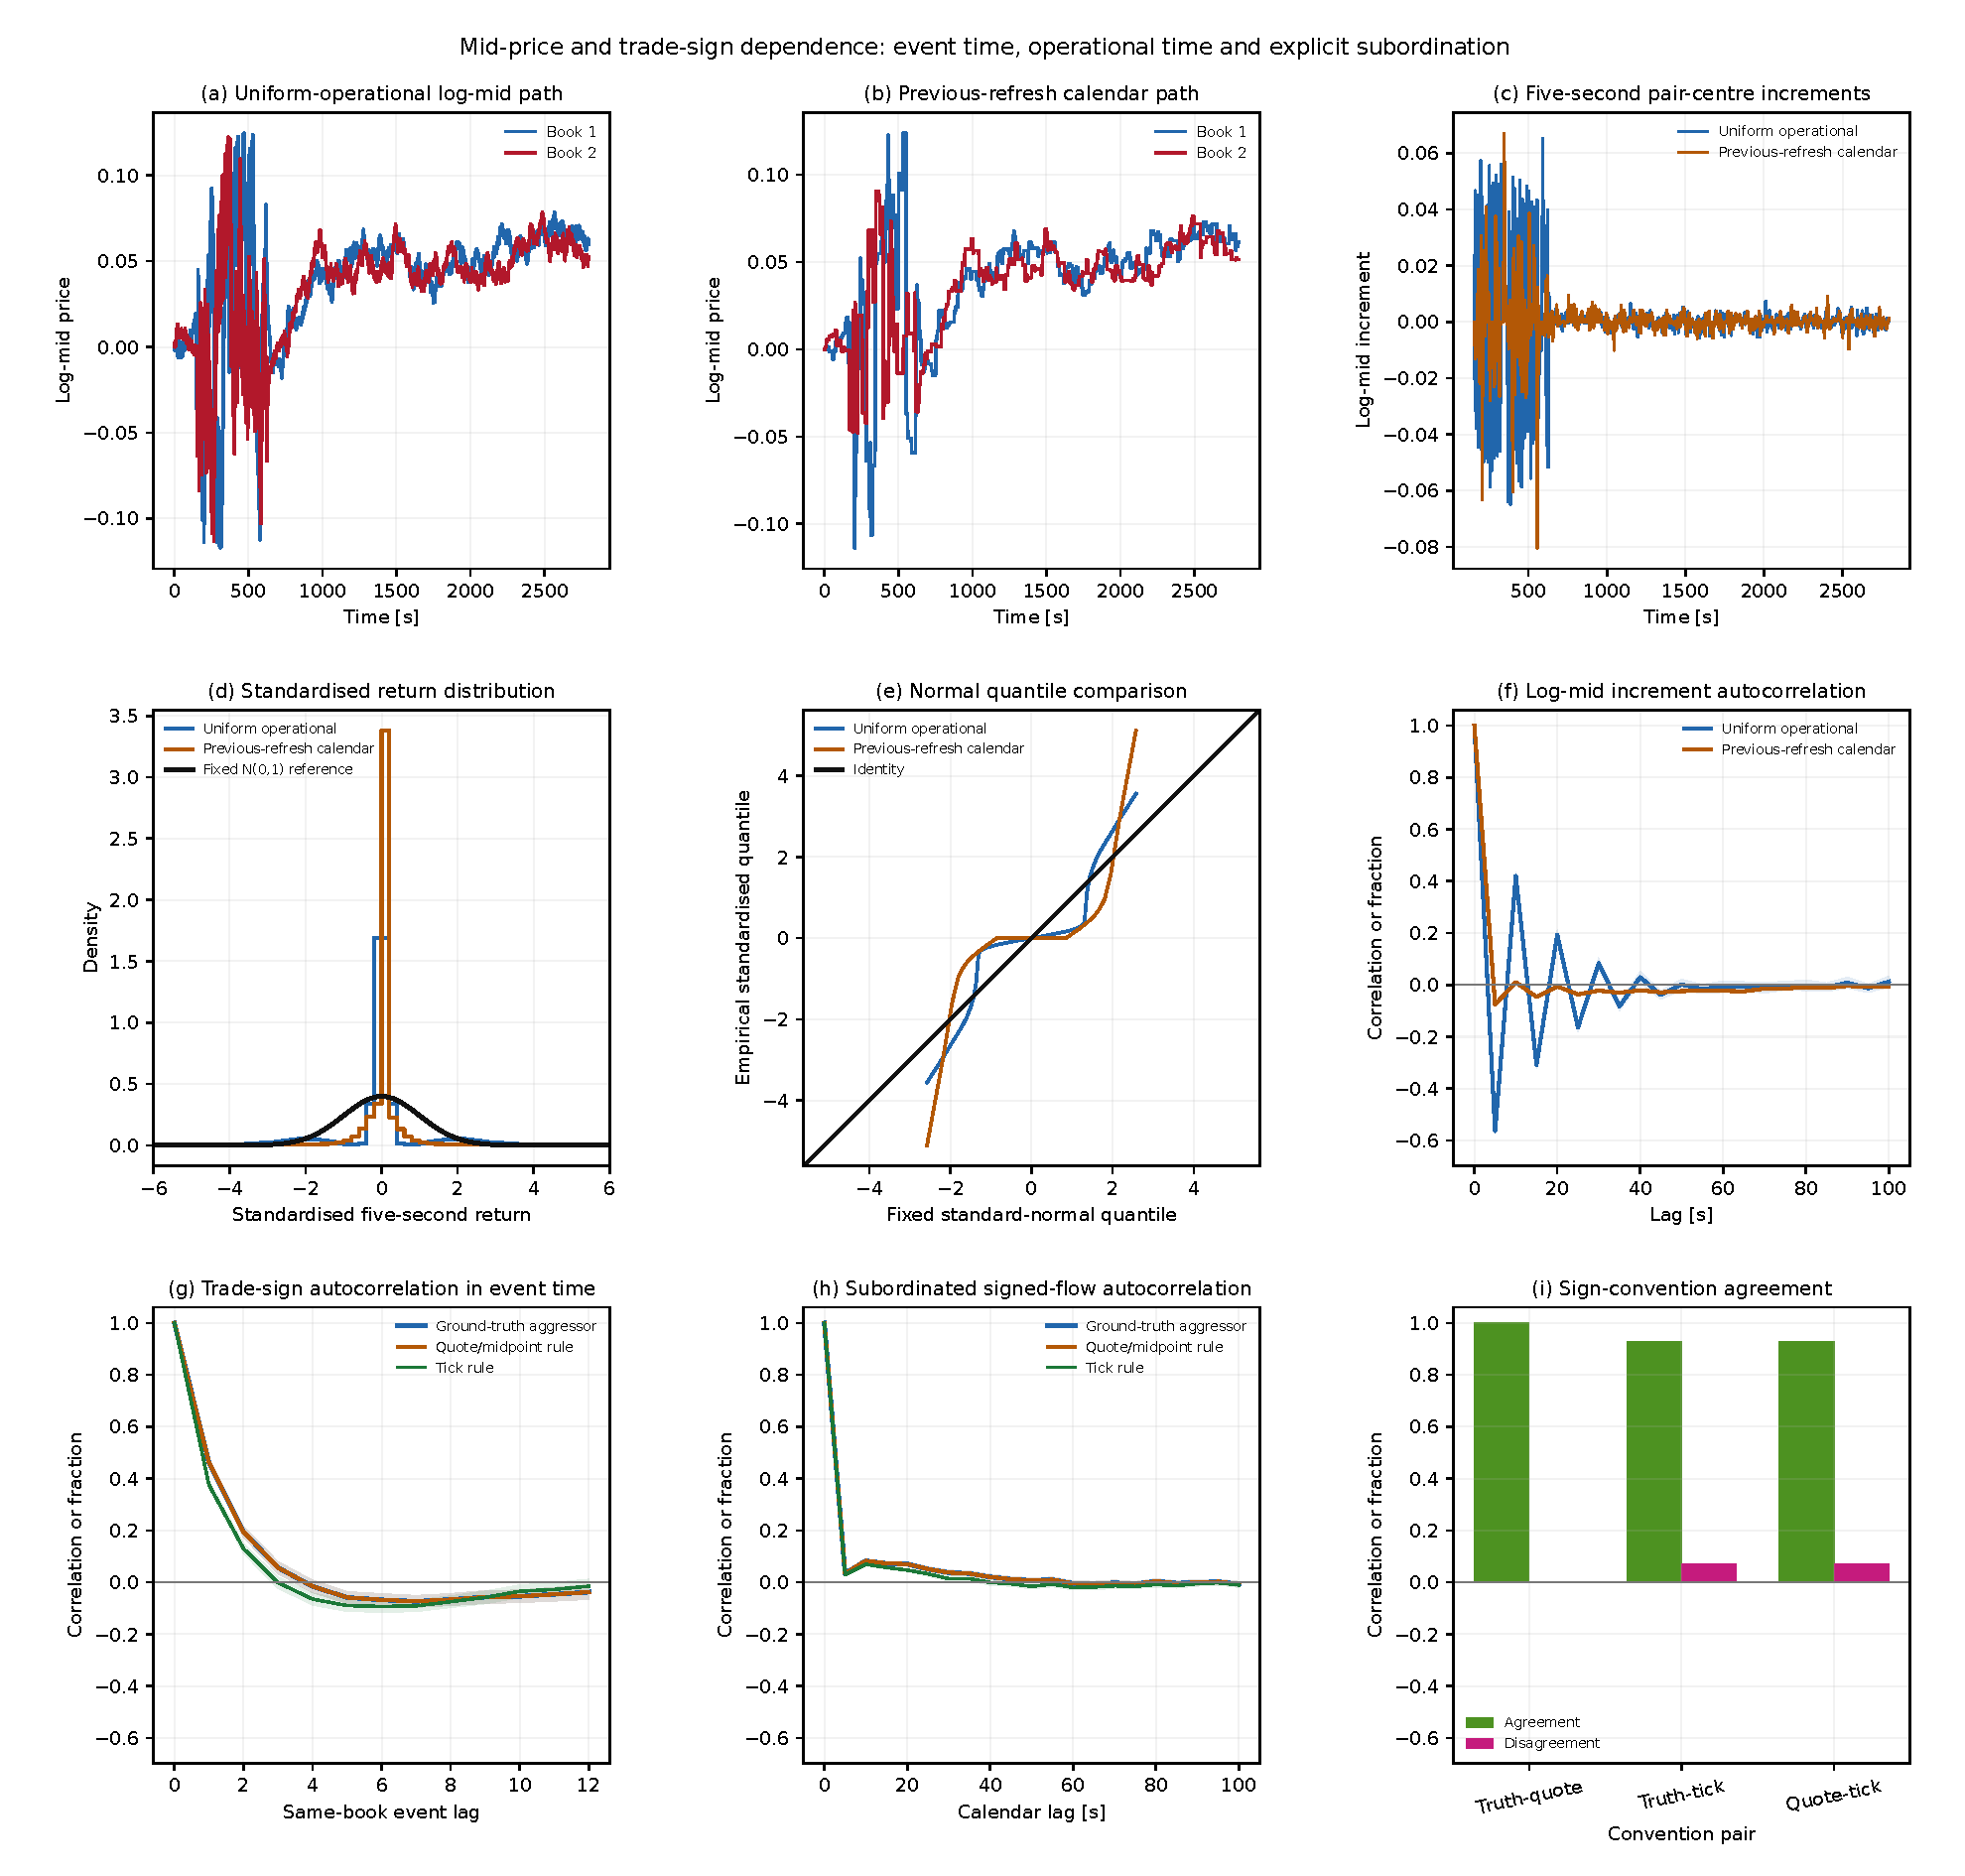
\includegraphics[width=\textwidth]{figures/figure-11-mid-price-trade-sign-autocorrelations-v2.pdf}
\caption{\textbf{Mid-price and trade-sign dependence.} The original nine-panel layout separates example paths and pair-centre increments (a--c), pooled standardized returns and normal quantiles (d--e), return autocorrelation (f), event-time sign autocorrelation (g), subordinated flow autocorrelation (h), and sign agreement (i). The example is the predeclared primitive group 2. Ensemble summaries use 128 independent primitive groups with explicit antithetic partners, 5600 half-second steps, $\Delta x=0.1$, and five-second returns after step 301. Each book has 48 quantity-0.015 events at the same fixed schedule; sign repeat probability is 0.75. Bands are pointwise 95\% intervals across independent groups. Extending the horizon adds post-execution time, so distributions and ACFs are horizon-dependent; periodic-schedule structure is not removed by smoothing. Normal curves are references, not fitted targets. These are finite-schedule diagnostics, not an endogenous long-memory claim.}
\label{fig:dependence}
\end{figure}

% Figure 12 supplementary-material insert for the v2.1.0 development gate.
% The published v2.0.0 supplement and accepted source-v1 paper remain frozen.

\subsection{Fixed-time order-book shock recovery}
\label{app:fixed-time-shock-recovery}

Figure~\ref{fig:fixed-time-shock-recovery} follows one buy market order in
book 1 through the current fixed-grid operational dynamics.  Immediately
before the declared operational step, the order consumes opposing density
from the reaction boundary outwards.  If $M_{1,n_*}$ denotes the resulting
density increment, then
\begin{equation}
  \varphi^+_{1,n_*}=\varphi^-_{1,n_*}+M_{1,n_*},
  \qquad
  \Delta x\sum_i |M_{1,n_*,i}|=Q.
\end{equation}
The event is applied once and only to book 1.  The second book remains active
through the receiving-front translation-mode coupling, although its density
and the coupling contribution are not separately drawn.

For a completed operational step the stored density satisfies
\begin{equation}
  \varphi_{j,n+1}
  =H_{j,n}+\varphi^+_{j,n}+C_{j,n}+A_{j,n}+L_{j,n}+B_{j,n},
\end{equation}
where $H$ is the transport or memory contribution,
\begin{equation}
  A_{j,n}=\Delta u\,q_j,
  \qquad
  C_{j,n}=\left(e^{-\nu_j\Delta u}-1\right)\varphi^+_{j,n},
  \qquad
  L_{j,n}=\Delta u\,\ell_{j\leftarrow k},
\end{equation}
and $B$ is the imposed outer-boundary correction.  The plotted arrivals,
removals and market-order impulse are density contributions rather than rates.
All are drawn on the same density scale.  In particular, the green curve is
$A_{j,n}=\Delta u\,q_j$ and is small relative to $\varphi_j$ because
$\Delta u=0.005$; it is not independently rescaled.  The unplotted terms are
retained in the machine-readable ledger.

Two differences from Bauer et al. Figure 2 follow from the present model.  The
accepted configuration has $\nu_1=\nu_2=0$, so $C_{j,n}=0$ and the gold
removal curve is identically zero.  It is retained to preserve the plotted
object map; no positive cancellation rate is introduced for visual agreement.
Second, boundary-outward consumption produces a short zero-density interval in
the intermediate $0^+$ state.  That state has no unique simple zero crossing.
The marker in panel (b) is therefore the last registered boundary $p_1^-$;
the first completed fixed-grid step restores a unique registered reaction
boundary.  Later markers are independently recovered from the corresponding
density states.

The first completed step gives an own-boundary displacement of $0.0997$ in
log-price units.  The displacement reaches $0.111$ at $2$ seconds and then
decreases to $0.0160$ at $80$ seconds.  Thus the computed late state is
substantially relaxed but remains displaced from the matched control over the
displayed horizon.

The calculation uses fixed $\Delta x=0.1$ and $\Delta u=0.005$ model-time
units, with $100$ seconds per model-time unit.  Innovations are set to zero so
that the chronology isolates event consumption, diffusion, source renewal and
coupling.  A matched no-event control remains in the numerical checks but is
not added to the nine-panel figure.  The result recovers the structure and
scientific question of the earlier figure; it does not assert numerical
identity with its non-uniform-time trajectory or parameterisation.

\begin{figure}[p]
\centering
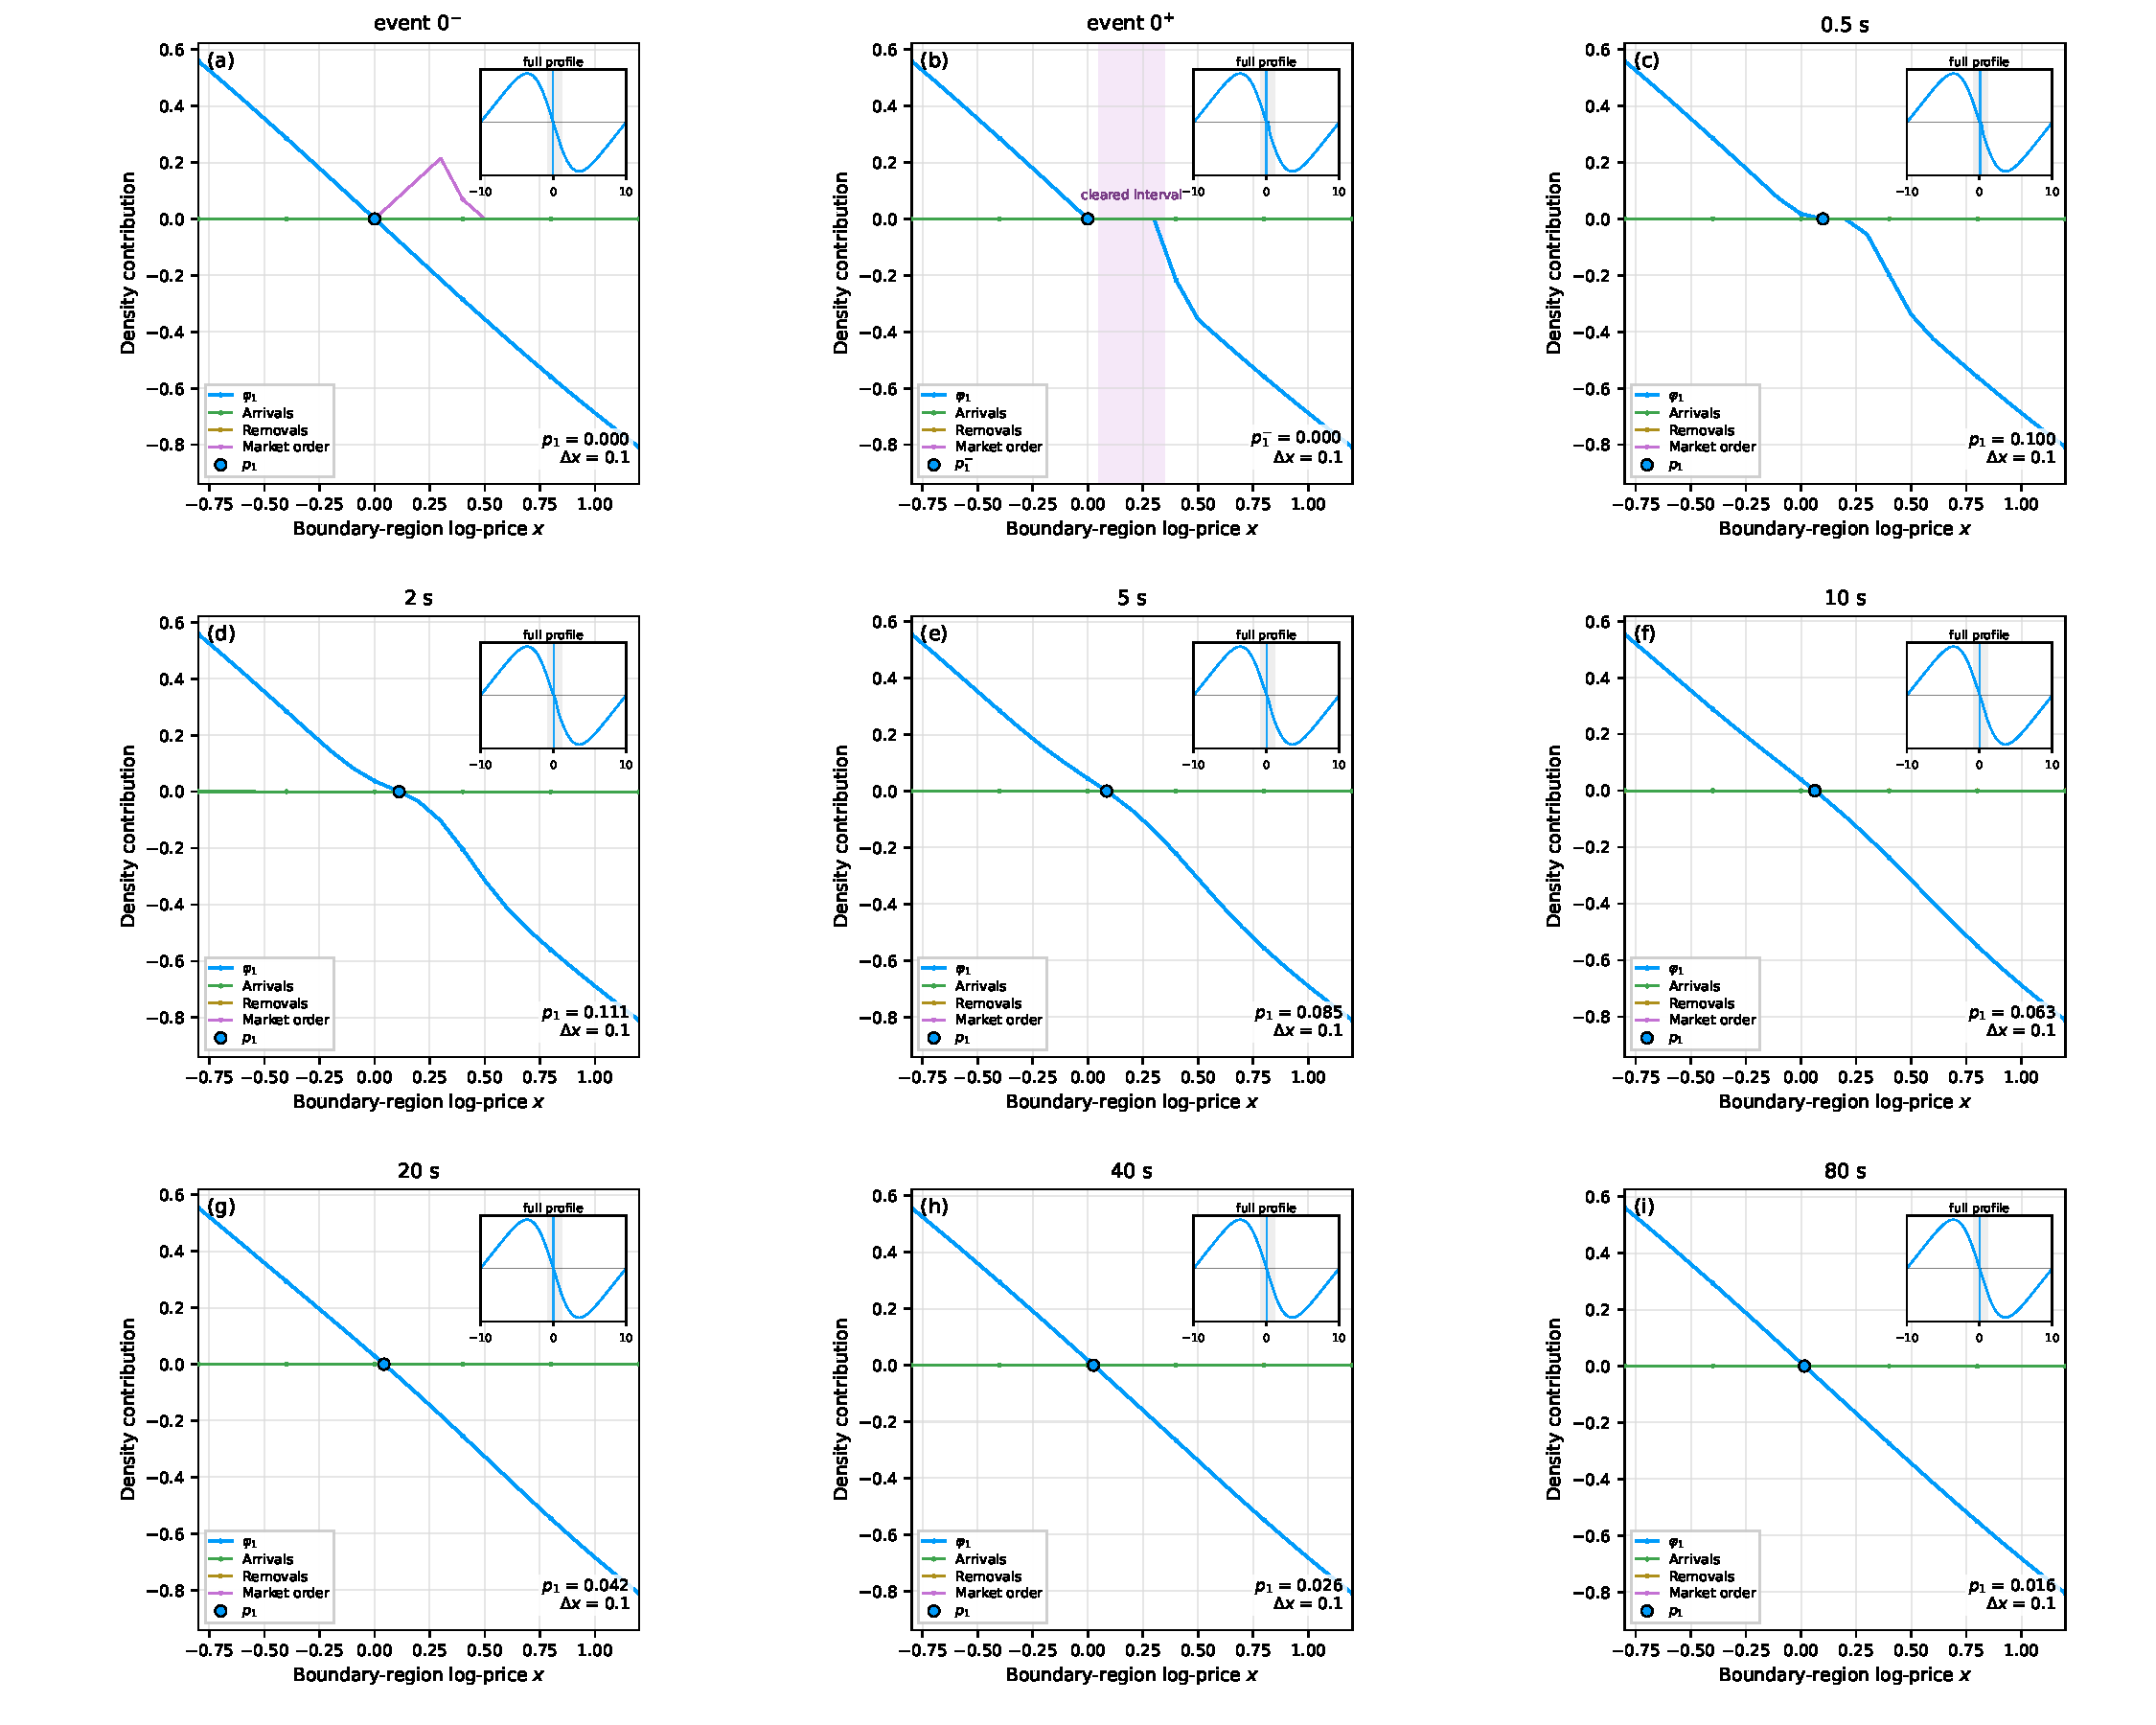
\includegraphics[width=\textwidth]{figures/figure-12-order-book-shock-recovery-v2.pdf}
\caption{\textbf{Fixed-time order-book shock recovery.} Nine snapshots follow
a buy market order in book 1 from the pre-event state $0^-$, through the
post-consumption state $0^+$, to $80$ seconds of fixed operational-time
evolution.  Blue is the signed density $\varphi_1$, green is the per-step
arrival contribution, gold is the per-step removal contribution, magenta is
the market-order density increment shown in panel (a), and the blue marker is the registered
reaction boundary.  The order consumes opposing liquidity from the boundary
outwards.  In panel (b) this creates a zero-density interval, so the marker is
the last registered boundary $p_1^-$; a unique simple zero is again registered
after the first completed step.  The accepted model has $\nu_1=\nu_2=0$, and
the gold curve is consequently zero in every panel.  Translation-mode coupling
to book 2 remains active and is retained in the numerical ledger but is not
drawn as an additional curve.  The registered boundary moves by $0.0997$ after
the first completed step, reaches $0.111$ at $2$ seconds and relaxes to a
residual displacement of $0.0160$ at $80$ seconds.  The price grid and
operational step are fixed.  All contribution curves use the same density
scale and are not independently rescaled.
The figure recovers the earlier panel structure without claiming a pointwise
replication of the Bauer et al. trajectory.}
\label{fig:fixed-time-shock-recovery}
\end{figure}


\clearpage

\subsection{Long-memory order flow and observation-clock morphology}
\label{app:stylised-facts-recovery}

Figure~\ref{fig:stylised-facts-recovery} separates two mechanisms that can
otherwise be confused.  The operational solver produces one completed pair of
price paths on the fixed grid.  Its innovations are Gaussian, while the
declared market-order signs are an exogenous order-splitting input.  Independent
book-specific renewal clocks are then applied by the exact previous-refresh
map in Eq.~\eqref{eq:subordination}.  Thus ``Gaussian'' labels the operational
innovations and never a waiting-time distribution.

For each primitive path and book, signs are constant over iid meta-order run
lengths $L$ with tail exponent $\nu=1.5$ and minimum run length two events;
successive run signs are iid and symmetric.  In the corresponding ideal
renewal construction the sign covariance decays as a power law proportional
to $k^{1-\nu}$.  This is a declared long-memory input motivated by order
splitting, not an endogenous consequence of the order-book dynamics and not an
empirical calibration.

The four rows hold the operational dynamics, event tape and query grid fixed.
They differ only in observation:
\begin{enumerate}
\item the completed operational path itself;
\item exponential waiting intervals with rate $0.1\,\mathrm{s}^{-1}$;
\item Mittag--Leffler waiting intervals with $\beta=0.8$ and
  $\tau=10\,\mathrm{s}$; and
\item the exact exponential tilt of that Mittag--Leffler law with
  $\lambda_T=0.0125\,\mathrm{s}^{-1}$.
\end{enumerate}
The resulting zero-return proportions at the five-second query scale are,
respectively, $0$, $0.6063$, $0.9097$ and $0.6648$.  The central spike, QQ
plateau and apparent tail thickening therefore measure observation-clock
morphology.  Untempered subdiffusion produces the longest holds; tempering
reduces, but does not remove, that effect.  A constant finite-horizon sampled
series is retained in distribution and impact averages, but its undefined ACF is not assigned an artificial value. Group ACFs require both books and both antithetic partners to be defined. At the longest horizon, the Mittag--Leffler row has between 121 and 125 of 128 valid groups, depending on lag and observable; this conditional availability is distinct from the unconditional return distribution.

\begin{figure}[p]
\centering
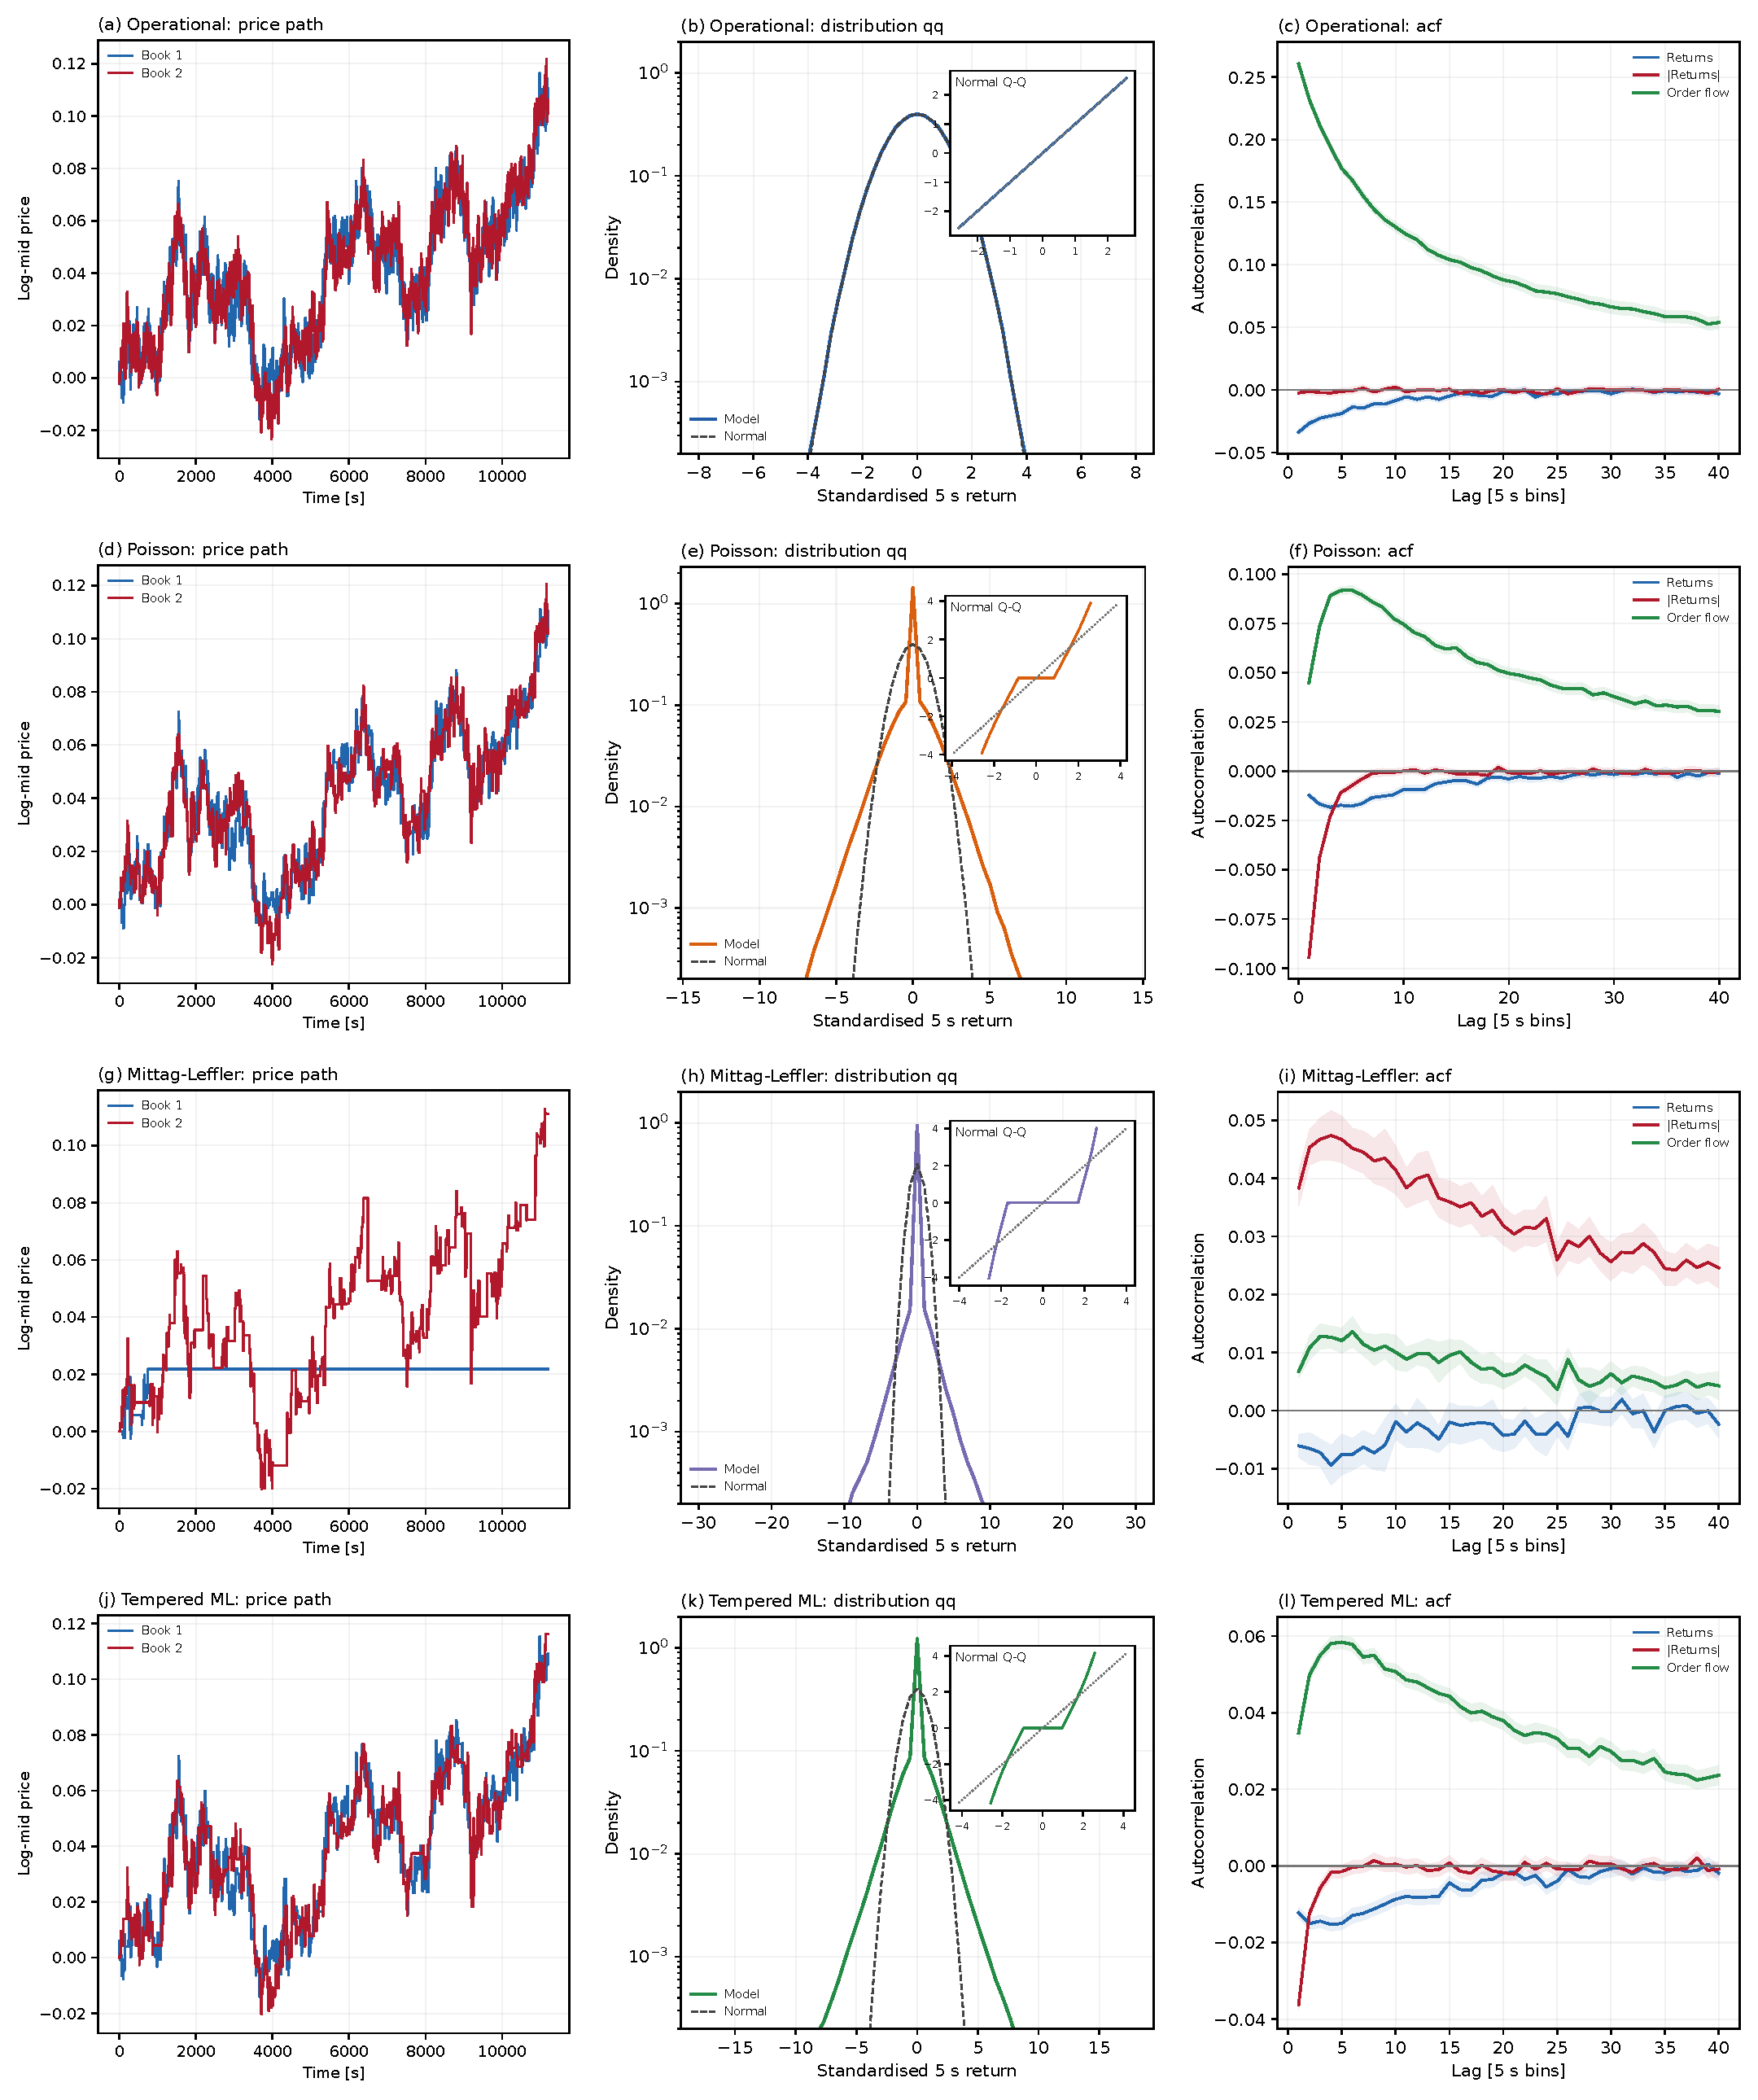
\includegraphics[width=\textwidth,height=0.74\textheight,keepaspectratio]{figures/figure-13-stylised-facts-recovery-v2.pdf}
\caption{\textbf{Operational long-memory input and observation-clock morphology.} The four rows show operational, Poisson, Mittag--Leffler and tempered Mittag--Leffler observation. The left column is the predeclared primitive group-2 path, with blue/red denoting books 1/2. The centre column shows pooled standardized five-second return densities on a logarithmic scale, with a fixed normal reference and QQ insets. The right column shows return (blue), absolute-return (red) and declared-flow (green) ACFs at lags in five-second bins; shading is pointwise 95\% mean uncertainty. Summaries use 128 independent groups with explicit antithetic partners, 22400 half-second steps and $\Delta x=0.1$. Exogenous quantity-0.0002 events arrive with probability 0.05 per step and Pareto sign-run exponent 1.5; only the longest horizon has the terminal 149-step no-event margin. Clocks start at time zero. Infinite-mean renewal aging makes observation-window length material. Constant paths remain in densities; undefined ACFs are omitted only at the declared complete-group level. Gaussian innovations do not require Gaussian observed returns, and no tail or clock parameters are refitted.}
\label{fig:stylised-facts-recovery}
\end{figure}


\clearpage
\input{source/source-v2/LONG-MEMORY-CLOCK-IMPACT-v2.2.0.tex}

\clearpage
\begin{landscape}
% Standalone table fragment. Required packages: booktabs, tabularx, array, float.
\begin{table}[H]
\centering
\scriptsize
\caption{\textbf{Parameter, timescale and identifiability register.} The table maps paper notation to implementation names and records units, roles, sensitivity pathways, and fixed or swept status. Refresh rate and source amplitude receive different code names despite source-notation overlap. Identifiability classifications describe the information available from the planned outputs under the stated model; they are not estimates, formal statistical-identifiability proofs, or empirical calibration results.}
\label{tab:parameter-register}
\renewcommand{\arraystretch}{0.98}
\begin{tabularx}{\linewidth}{@{}p{1.7cm}p{3.3cm}p{2.3cm}p{2.5cm}X X X X@{}}
\toprule
Paper symbol & Code name & Source & Units & Role & Sensitivity path & Figure treatment & Identifiability from Epps output \\
\midrule
\(\Delta\) & \texttt{aggregation\_\allowbreak{}scale} & Eqs. (8), (9), (11) & time; dimensionless after scaling & return aggregation horizon & direct horizontal scale & swept in F1-F6 & observed/design variable \\
\(\rho_\infty\) & \texttt{rho\_\allowbreak{}inf} & Eqs. (8), (9), (11) & dimensionless correlation & long-scale vertical level & multiplicative vertical scale & fixed to one in base figures & conditional on plateau coverage \\
\(\lambda_{12}\) & \texttt{clock\_\allowbreak{}rate} & Eq. (8); App. A & time\(^{-1}\) & pooled refresh/overlap rate & \(F(\lambda_{12}\Delta)\) & unit scale; sensitivity in F2 & conditional; independently measurable in v2 \\
\(\kappa=\kappa_1+\kappa_2\) & \texttt{response\_\allowbreak{}rate} & Eq. (9); App. B & time\(^{-1}\) & spread relaxation rate & \(F(\kappa\Delta)\) & swept in F1-F2; derived in F4-F5 & conditional on clock rate and short scales \\
\(\alpha_c\) & \texttt{alpha\_\allowbreak{}clock} & App. C, Eq. (C.18) & dimensionless & fractional clock order & short power \(\Delta^{\alpha_c}\) & swept in F3 & not separate from alpha\_response at short scale \\
\(\alpha_r\) & \texttt{alpha\_\allowbreak{}response} & App. C, Eq. (C.18) & dimensionless & fractional response order & short power \(\Delta^{\alpha_r}\) & swept in F3 & not separate from alpha\_clock at short scale \\
\(\tau_c,\tau_r\) & \texttt{clock\_\allowbreak{}characteristic\_\allowbreak{}time}\newline\texttt{response\_\allowbreak{}characteristic\_\allowbreak{}time} & v1 nondimensionalisation & time & fractional scale convention & \((\Delta/\tau)^\alpha\) & fixed to one in F3 & confounded with fractional rate convention \\
\(\gamma_{jk}\) & \texttt{coupling\_\allowbreak{}strength} & Eq. (6); App. B & model-dependent & pair-trader coupling strength & \(\kappa_j\propto\gamma_{jk}\) & one-at-a-time sweep in F4 & not separate from source/front quantities \\
\(\lambda_j\) (source) & \texttt{source\_\allowbreak{}amplitude} & Eq. (5); App. B & source amplitude & decaying-Gaussian amplitude & \(M_j^+\propto a_j\) & one-at-a-time sweep in F4 & not separate from coupling strength \\
\(\mu_j\) & \texttt{source\_\allowbreak{}width} & Eq. (5); App. B & price\(^{-2}\) & Gaussian source-shape scale & \(M_j^+\propto\mu_j^{-1/2}\) & one-at-a-time sweep in F4 & not separate from amplitude/front slope \\
\(|\mathcal L_j|\) & \texttt{front\_\allowbreak{}slope\_\allowbreak{}abs} & Eq. (B.9); Eq. (B.13) & density per price & frozen reaction-front slope & \(\kappa_j\propto|\mathcal L_j|^{-1}\) & one-at-a-time sweep in F4 & not identifiable as thickness from Epps alone \\
\(\varepsilon\) & \texttt{epsilon} & Eq. (6); App. D & price\(^2\) for \(yz/\varepsilon\) & continuum selector regularisation & centred moment invariant; representation path & swept in F5 & not a reaction-front thickness parameter \\
\(\Delta x\) & \texttt{lattice\_\allowbreak{}spacing} & App. D & price & numerical lattice resolution & discrete moment error to effective response & swept in F5 & known numerical control \\
\(z_{jk}\) & \texttt{directed\_\allowbreak{}spread} & Eq. (6); App. B & price & directed book-price spread & selector argument \(yz/\varepsilon\) & fixed to 0.2 in F5 & state variable, not inferred parameter \\
-- & \texttt{alignment\_\allowbreak{}offset\_\allowbreak{}cells} & v1 numerical diagnostic & lattice cells & source-selector centring error & parity breaking to effective response & 0 and 0.5 in F5 & known numerical control \\
-- & \texttt{domain\_\allowbreak{}halfwidth} & v1 numerical diagnostic & price & finite integration/lattice domain & tail truncation to effective response & full and truncated in F5 & known numerical control \\
\bottomrule
\end{tabularx}
\end{table}

\end{landscape}

\begin{landscape}
\input{tables/table-02-numerical-benchmarks-v2.2.0.tex}
\end{landscape}

\section{Parameter and numerical evidence}

Table~\ref{tab:parameter-register} keeps the source notation, unambiguous code names, units, sensitivity paths, and identifiability qualifications together. In particular, the paper's refresh-rate and source-amplitude uses of \(\lambda\) are separated in code. Table~\ref{tab:numerical-benchmarks} retains the published deterministic diagnostic results and tolerances; it does not certify the new stochastic precision or continuum limit. The fractional reference points were computed independently with adaptive quadrature, while the release evaluator uses fixed composite Gauss--Legendre quadrature and a small-argument series.

\section{Numerical resolution and reproducibility}

\begin{center}
\small
\begin{tabularx}{\textwidth}{@{}p{2.7cm}p{2.5cm}X@{}}
\toprule
Comparison & Independent groups & Resolution and uncertainty \\
\midrule
Clock and coupling (7a--c) & 512 validation & 8000 s after 200 s warm-up; $\Delta x=0.1$, 0.5 s update; 98\% pointwise ratio intervals. \\
Impact (9, 10, 14) & 512 primitive & $\Delta x=0.05$, 0.125 s update; 161 lag points; 95\% pointwise mean intervals. \\
Finite-schedule dependence (11) & 128 primitive & 5600 half-second steps; explicit antithetic partners; 95\% pointwise intervals. \\
Persistent-flow morphology (13) & 128 primitive & 22400 half-second steps; explicit antithetic partners; 95\% pointwise intervals where defined. \\
\bottomrule
\end{tabularx}
\end{center}

The short-lag grid comparison is discussed with Eq.~\eqref{eq:discrete-coupling}; it does not change the following precision statements for the previously sampled ranges. At the original 95\% precision criterion, the clock-only maximum half-width is 0.00182. Coupling-only and combined half-widths are 0.00631 and 0.00604, exceeding the proposed 0.002 target. Nineteen of 24 impact schedule--clock--response combinations meet the fixed plot-scale precision criterion; five, primarily involving renewal-clock cross impact, remain above it. These results are retained without changing seeds or fitting parameters. The finer $\Delta x=0.025$ impact screen still changes early own impact by approximately 0.001--0.003; the production $\Delta x=0.05$ grid is not a certified continuum limit. The 128-group persistent-flow study meets its longest-horizon positive-lag ACF precision targets, but finite-schedule and horizon effects remain.

The source boundary is the published v2.1.0 commit
\texttt{e932f7c66449d4fd5e0269cbcaafa324d91b51bf}.
The numerical figures are regenerated from the declared settings and fixed seeds through the existing entry point:
\begin{verbatim}
python scripts/run_all.py
\end{verbatim}
To compile this supplement from the repository root, run the following command twice:
{\small
\begin{verbatim}
pdflatex -output-directory=supplementary-materials SUPPLEMENTARY-MATERIAL-v2.2.0.tex
\end{verbatim}
}
Document compilation uses the generated figures; it does not rerun simulations.

The retained figures are verified against their immutable supplied assets. The full v2.1.0 release remains available independently. PDF bytes may differ across renderers, fonts and platforms; machine-readable values, seed rules, input hashes, tolerances and declared statistical units are the scientific reproducibility objects. The source asset and its accepted data are preserved.

\section{Interpretive limits}

The diagnosed computations support a limited set of conclusions. Ordinary clock and coupling factors are distinguishable when their timescales are sufficiently separated and the components are shown explicitly. The long-scale plateau contains little local information about either rate. Within the stated fractional product ansatz, the leading short-scale power identifies an order sum rather than two separate orders; this is not a general result for a joint clock--coupling process. Reaction-boundary quantities affect the Epps curve conditionally through the effective response rate, but are not individually identified by that curve. Continuum selector invariance can coexist with finite-grid distortion when parity, alignment or domain controls are not respected. The clock-only matched statistic is close to its theoretical factor at the plotted scale. Coupling comparisons retain short-scale residuals, and the combined product is a separability approximation with a different short-time power from the joint reduced process. Reduced conditional moments account for realized clock indices without proving identity with the full reaction--diffusion process. Heavy-tailed sign runs establish a controlled long-memory input but do not show that the book endogenously generates that memory. Mittag--Leffler clocks change observed return morphology and delay observed impact without changing the underlying operational response. The impact, shock-recovery, autocorrelation and stylised-facts figures are conditional model diagnostics, not empirical calibration.

These are computational illustrations and numerical verification statements inside the paper's assumptions. They are not empirical validation, calibration or proof of the approximations. The antecedent implementation is not required to execute or interpret these comparisons.

\medskip
\noindent\textbf{Software and licensing note.} Code is provided under the MIT License; supplementary text, captions, generated figures, tables, and documentation are provided under CC BY 4.0. The paper and frozen source retain their existing terms.

\end{document}
